\documentclass[oneside,a4paper]{book}
%\pagestyle{headings}
\frontmatter
%=============================================================================

\usepackage{amsthm}
\usepackage{xspace}
\usepackage{float}
\usepackage{ifthen}
\usepackage{amsbsy}
\usepackage{amssymb}
\usepackage{balance}
\usepackage{booktabs}
\usepackage{graphicx}
\usepackage{rotating}
\usepackage{multirow}
\usepackage{needspace}
\usepackage{microtype}
\usepackage{bold-extra}
\usepackage{geometry}
\usepackage{varioref}
\usepackage{xcolor}
\usepackage{textcomp}
\usepackage{listings}
\usepackage[normalem]{ulem} %emphasize still italic
\usepackage{ucs}

\usepackage[latin1]{inputenc}
\usepackage[htt]{hyphenat}
\usepackage{times}
\usepackage{url}
\usepackage{alltt}
\usepackage{amsmath}
\usepackage{xfrac}
\usepackage{subfigure}
\usepackage{appendix}
\usepackage{stmaryrd}   % for the \shortuparrow
\usepackage[utopia]{quotchap}

\usepackage{setspace}
\usepackage[numbers, sort&compress]{natbib}
\usepackage{mdwlist}        % support for better spaced lists
% allows for temporary adjustment of side margins
\usepackage{chngpage}
\usepackage[normalem]{ulem} 

% constants

\newcounter{qcounter}

% commands
\newcommand{\n}{$\cdot$}
\newcommand{\y}{\checkmark}
\newcommand{\subscript}[1]{$_{\textrm{\footnotesize{#1}}}$}
\newcommand{\superscript}[1]{$^{\textrm{\footnotesize{#1}}}$}
\newcommand{\vertical}[1]{\raisebox{-4em}{\begin{sideways}{#1}\end{sideways}}}

\newboolean{showedits}
\setboolean{showedits}{true} % toggle to show or hide edits
\ifthenelse{\boolean{showedits}}
{
       \newcommand{\ugh}[1]{\textcolor{red}{\uwave{#1}}} % please rephrase
       \newcommand{\ins}[1]{\textcolor{blue}{\uline{#1}}} % please insert
       \newcommand{\del}[1]{\textcolor{red}{\sout{#1}}} % please delete
       \newcommand{\chg}[2]{\textcolor{red}{\sout{#1}}{\ra}\textcolor{blue}{\uline{#2}}} % please change
}{
       \newcommand{\ugh}[1]{#1} % please rephrase
       \newcommand{\ins}[1]{#1} % please insert
       \newcommand{\del}[1]{} % please delete
       \newcommand{\chg}[2]{#2}
}


% ============================================================================
% Put edit comments in a really ugly standout display

\usepackage{xcolor}
\usepackage[normalem]{ulem}
\newcommand{\ra}{$\rightarrow$}


% comments \nb{label}{color}{text}
\newboolean{showcomments}
\setboolean{showcomments}{true}
\ifthenelse{\boolean{showcomments}}
    {\newcommand{\nb}[3]{
        {\colorbox{#2}{\bfseries\sffamily\scriptsize\textcolor{white}{#1}}}
        {\textcolor{#2}{\sf\small$\blacktriangleright$\textit{#3}$\blacktriangleleft$}}}
     \newcommand{\version}{\emph{\scriptsize$-$Id$-$}}
%	 \newcommand{\ugh}[1]{\textcolor{red}{\uwave{#1}}} % please rephrase
%	 \newcommand{\ins}[1]{\textcolor{blue}{\uline{#1}}} % please insert
%	 \newcommand{\del}[1]{\textcolor{red}{\sout{#1}}} % please delete
%	 \newcommand{\chg}[2]{\textcolor{red}{\sout{#1}}{\ra}\textcolor{blue}{\uline{#2}}} % please change
	 \newcommand{\chk}[1]{\textcolor{ForestGreen}{#1}} % changed, please check
	}
    {\newcommand{\nb}[3]{}
     \newcommand{\version}{}
	\newcommand{\chk}[1]{} % changed, please check
	}

% ============================================================================
% Make quotes be italic
\renewenvironment{quote}
    {\list{}{\rightmargin\leftmargin}%
     \item\relax\begin{it}}
    {\end{it}\endlist}

\newcommand{\ttimes}{\ensuremath{\times}}

%=============================================================================

\newcommand{\needlines}[1]{\Needspace{#1\baselineskip}}

% source code
\usepackage{xcolor}
\usepackage{textcomp}
\usepackage{listings}
\definecolor{source}{gray}{0.9}
\lstset{
	language={},
	% characters
	tabsize=3,
	upquote=true,
	escapechar={!},
	keepspaces=true,
	breaklines=false,
	alsoletter={:},
	breakautoindent=true,
	columns=fullflexible,
	showstringspaces=false,
	basicstyle=\footnotesize\ttfamily,
	% background
	frame=single,
    framerule=0pt,
	backgroundcolor=\color{source},
	% numbering
	numbersep=5pt,
	numberstyle=\tiny,
	numberfirstline=true,
	% captioning
	captionpos=b,
	numberbychapter=false,
	% formatting (html)
	moredelim=[is][\textbf]{<b>}{</b>},
	moredelim=[is][\textit]{<i>}{</i>},
	moredelim=[is][\uline]{<u>}{</u>}}
\newcommand{\ct}{\lstinline[backgroundcolor=\color{white},basicstyle=\footnotesize\ttfamily]}
\newcommand{\lct}[1]{{\small\tt #1}}


%----------------------------------------------------------------------------
% references
\newcommand{\tabref}[1]{\hyperref[{tab:#1}]{Table~\ref*{tab:#1}}}
\newcommand{\figref}[1]{\hyperref[{fig:#1}]{Figure~\ref*{fig:#1}}}
\newcommand{\secref}[1]{\hyperref[{sec:#1}]{Section~\ref*{sec:#1}}}
\newcommand{\lstref}[1]{\hyperref[{lst:#1}]{Listing~\ref*{lst:#1}}}
\newcommand{\charef}[1]{\hyperref[{cha:#1}]{Chapter~\ref*{cha:#1}}}
%----------------------------------------------------------------------------

% abbreviations
\tracingcolors 4
\setcounter{tocdepth}{3}
\setcounter{secnumdepth}{3}
\newcommand{\ie}{\emph{i.e.,}\xspace}
\newcommand{\eg}{\emph{e.g.,}\xspace}
\newcommand{\etc}{\emph{etc.}\xspace}
\newcommand{\etal}{\emph{et al.}\xspace}


\newcommand{\newevenside}{
	\ifthenelse{\isodd{\thepage}}{\newpage}{
	\newpage
        \phantom{placeholder} % doesn't appear on page
	\thispagestyle{empty} % if want no header/footer
	\newpage
	}
}

\def\stretchfactor{1}
\newcommand{\mychapter}[1]{\setstretch{1}
    \chapter{#1}\setstretch{\stretchfactor}}

%----------------------------------------------------------------------------
\newcommand{\lessSpace}{\vspace{-1em}}
\DeclareGraphicsExtensions{.pdf,.png}
\graphicspath{{images/}}
\newcommand{\fig}[4]{
	\begin{figure}[#1]
		\centering
		\includegraphics[width=#2\textwidth]{#3}
		\lessSpace
		\caption{\label{fig:#3}#4}
	\end{figure}}

% ===========================================================================

%:CONFIGURE THIS

\usepackage{tikz}
\usetikzlibrary{arrows,decorations.pathmorphing,backgrounds,fit,positioning,shapes.symbols,chains,shapes.geometric,shapes.arrows,calc}
\usepackage[simplified]{pgf-umlcd}

\usepackage{pdflscape}
\usepackage{fontawesome5}
\usepackage{wasysym}

\newcommand{\cfigureCaption}{}
\newenvironment{cfigure}[2][]{
	\begin{figure}
	\centering
	\renewcommand{\cfigureCaption}{\label{#1}#2}
}{
	\lessSpace
	\caption{\cfigureCaption}
	\end{figure}
}

\newenvironment{instructions}{
	\begin{list}{$\rightarrow$}{}
}{
	\end{list}
}

\newenvironment{todo}{
	\PackageWarning{ToDo}{!!! Unresolved issues !!!}
	\begin{list}{\faTasks}{}
}{
	\end{list}
}

\lstnewenvironment{code}{%
	\lstset{%
		% frame=lines,
		frame=single,
		framerule=0pt,
		mathescape=false
	}
}{}

% \bibliographystyle{plainnat}

\newcommand{\thesistitle}{Revealing Programming Language Abstractions}
\newcommand{\thesisauthor}{Simon B�nzli Straub}
\newcommand{\thesisauthorOrigin}{Bern, Switzerland}
\newcommand{\thesisleiter}{Prof.\ Dr.\ Timo Kehrer, Prof.\ Dr.\ Oscar Nierstrasz}
\newcommand{\thesisasst}{}
\newcommand{\thesisurl}{http://seg.inf.unibe.ch/}
\newcommand{\thesissubtitle}{An Excerpt of nand-to-tetris -- in Reverse -- Using Smalltalk}
\newcommand{\thesisdate}{15. August 2025}

% ===========================================================================

\usepackage[ colorlinks=true, urlcolor=black, linkcolor=black,
			citecolor=black, bookmarksnumbered=true, bookmarks=true,
			plainpages=false,
			pdftitle={\thesistitle}, pdfauthor={\thesisauthor},
			pdfsubject={\thesissubtitle}, pdfpagelabels]{hyperref}

\newcommand{\hrref}[2]{\hyperref}
% ===========================================================================
% ===========================================================================

% D O C U M E N T
% % % % % % % % % % % % % % % % % % % % % % % % % % % % % % % % % %
\begin{document}

% T I T L E
% % % % % % % % % % % % % % % % % % % % % % % % % % % % % % % % % %
\begin{titlepage}  
  \begin{center}  
  
  \begin{figure}[t]  
  \vspace*{-2cm}        % to move header logo at the top 
  \center{
\includegraphics[scale=0.2]{logos/gyminf_logo.png}}
  \vspace{0.4in}     
  \end{figure}

    \thispagestyle{empty}
    
    {\bfseries\Huge \thesistitle \par
    \Large \vspace{0.1in} \thesissubtitle \par}

    \vspace{0.3in} 
    \LARGE{\textbf{GymInf Individual Project} \\}
    \vspace{0.4in}

    {\Large \thesisauthor \par from \par \thesisauthorOrigin}
    
    \vspace{0.3in}
    {\Large Philosophisch-naturwissenschaftlichen Fakult\"{a}t \\
            der Universit\"{a}t Bern \par}
    \vspace{0.3in}
    {\Large \thesisdate \par}
    \vspace{0.3in}
    %Leiter der Arbeit: \par
   {\Large \thesisleiter} \par
      {\Large \thesisasst} \par
   \vspace{0.1in}
    {\Large Software Engineering Group \par Institut f\"{u}r Informatik \par University of Bern, Switzerland \par}
  

  \vspace{0.9in}
 
  % === Logos ==============================================     
  \begin{figure}[htp]
    \centering
    
\includegraphics[scale=0.30]{logos/UNI_Bern.png}\hfill
    
\includegraphics[scale=0.30]{logos/UNI_Neuenburg.png}\hfill
    
\includegraphics[scale=0.80]{logos/UNI_Fribourg.png}
  \end{figure}
  % === // Logos ===========================================    


  \end{center}

\end{titlepage}

% A B S T R A C T
% % % % % % % % % % % % % % % % % % % % % % % % % % % % % % % % % %
\chapter*{\centering Abstract}
\begin{quotation}
\noindent

This thesis presents an environment to teach programming and computer architecture at high school level that allows students to experience and interactively explore various abstraction levels involved in running a program.

Didactic literature suggests that exploring different abstraction levels improves students' understanding of both programming and the inner workings of a computer system. Such multi-layered exploration is also considered a foundational idea of computer science and has to be taught because, among other reasons, some lower abstraction layers tend to leak through interfaces anyway.

For this purpose, the teaching environment ``Processing Abstractions'' has been created on the basis of the Smalltalk environment Glamorous Toolkit. This environment contains a compiler for a subset of the Processing programming language in its Python form, for which a variety of views were molded: tokenization, syntax tree building, transpilation of Processing into Smalltalk, translations to an intermediary language and eventually to Smalltalk bytecode, and finally, the program's actual output. These views are tied to the source code, updated live for seamless exploration, and can be composed into interactive material to teach the abstraction levels involved in programming; examples for which are also included.

Processing Abstractions has been used and evaluated during a few lessons. On the basis of the limited data available, the evaluation shows that the live environment does encourage experimentation and allows students to work and learn at their own pace and depth. However, understanding of the various layers has not improved significantly in the short period of time that the environment could be tested.

\end{quotation}
\clearpage


% C O N T E N T S
% % % % % % % % % % % % % % % % % % % % % % % % % % % % % % % % % % % % % % % %
\tableofcontents

\mainmatter

%%%%% Introduction %%%%%

\chapter{Introduction}

In modern digitized society, the importance of computer science has grown to the point where some of its subjects are taught at schools of all levels. Whereas elementary schools focus on introducing digital, connected devices and their applications, high schools also teach fundamentals. And while programming or application use courses have been implemented since decades ago, broader and more theoretical courses have recently become standard. \eg in Switzerland, computer science has become an obligatory subject for all high school students similar to more traditional sciences starting in 2019.

The curricula used at high schools usually contain introductions not only to algorithms and programming, but among others also into encodings, computer architecture, networking and social ramifications such as privacy and security (see \eg \cite{Erz16}). As such, students not only are taught a high level programming language such as Python, but should also have insights into what happens at various other abstraction layers when such a program is stored and run.

One traditional approach to teaching computer architecture consists in teaching a separate assembly-like language during the introduction to computer architecture. This can happen in a more gamified fashion \eg with ``Human Resource Machine'' \cite{Tom15}, closer to theory like ``Von Neumann Simulator'' \cite{Gan23} or even without mnemonics as using the Little Man Computer architecture \cite{Oin25}. While all of these approaches help to show how a microprocessor might approximately work, none of them offer a direct, explorable connection to a high level language.

In our experience, high level programming is quite well received with students, whereas the teaching sequence on computer architecture is less so. Programming and computer architecture also didn't fit together as nicely as we'd have liked and processor and memory remained a mystery for too many students. This lead us to look into a better way of combining the two:

One suggestion for such a direct connection between high level language and machine code will be presented in this thesis in form of a teaching environment targeted at high school students and implemented based on ``Glamorous Toolkit'' (introduced in section \ref{sc_gt}) for the ``Processing'' programming language based on Python syntax (which will be introduced in section \ref{sc_processing}).

We consider such a teaching environment being called for, if didactic literature (summarized in \ref{sc_didactic}) and currently existing \acp{IDE} are considered. In particular, we propose to use this as a basis for explicitly discussing the foundational idea of multitier abstractions with students which appear in multiple places all throughout their curriculum within computer science -- most prominently in networking and in information encoding -- but also in other subject matters such as natural sciences, psychology, \etc. This discussion is important insofar as the clean separation of abstraction layers may unexpectedly fail or ``leak'' (a concept introduced in \ref{ssc_leaky_abstractions}).

The teaching environment introduced in chapter \ref{ch_pa} of this thesis (named ``Processing Abstractions'') will focus in particular on abstractions encountered during programming (see \eg figure \ref{fig_screenshot_vm_execution} on page \pageref{fig_screenshot_vm_execution}), allowing students to have a \emph{Sichtenwechsel} on their own programs.

For teachers, suggestions for how to include it in the classroom are provided in chapter \ref{ch_teaching}, with a sequence on computer architecture at the center, but for embedding surrounded by two sequences on programming and compilers. All of these sequences build upon the teaching environment provided and rely on students being able to get multiple, varied views and insights into the same program, in order to experience the behind-the-scenes work or rather the details usually abstracted away in an interactive way. The student's engagement builds upon all input being readily modifiable with changes being immediately visible, allowing for almost frictionless exploration.

Parts of suggested lessons have already been implemented with two classes at the Gymnasium Neufeld in Berne for collecting valuable feedback from students. While the sample size was too small to get significant results, observations and student feedback (discussed in chapter \ref{ch_practice}) have shown that the environment works and that students are motivated by its liveness to explore the concepts provided. Whether their understanding of the abstraction levels involved have improved, could however unfortunately not (yet) be shown.

All of this wouldn't have been possible without the very helpful support of Prof.\,em. Oscar Nierstraz who has finally managed to introduce me to Smalltalk and Prof. Timo Kehrer who has taken this project together with his predecessor below his wing. I also want to thank my students from the classes 27Ga and 28Ga of Gymnasium Neufeld who have worked with my productions and given helpful feedback. Finally, many thanks go to my kids for their understanding of me having to work even during their holidays and to my wife for her endless support which made this thesis possible in the first place.

%%%%% The Problem %%%%% and %%%%% Related Work %%%%%

\chapter{State of the Art in Computer Science Didactics} \label{ch_theory}

With relation to systems, didactic literature recommends to examine multiple layers of a system, in order for students to better understand the material. This concept (later called \emph{Sichtenwechsel} for lack of a better fitting English term) is introduced in \ref{ssc_sichtenwechsel} and is considered a foundational idea which should be taught explicitly (elaborated in \ref{ssc_fundamentale_ideen}).

Learning to handle complex systems is at the core of what happens in many subjects in school (high school and beyond). With relation to computer science, this is asked for in particular when teaching students ``computational thinking'' (see \ref{ssc_ct}). One aspect that we feel is particularly important in this regard is the fact that systems can rarely be separated into independently investigable layers in a clean way -- or in other words: many abstractions involved in layering complex systems leak (see \ref{ssc_leaky_abstractions}).

When multiple abstraction layers are taught together, common approaches consist in doing so either bottom up (\ref{ssc_bottom_up}) or top down (\ref{ssc_top_down}), showing how to potentially proceed.

In our experience, one thing high school students like particularly well during their computer science curriculum is programming (which is reflected in student feedback discussed in chapter \ref{ch_practice}). Therefore, we want to merge the discussion on multitier abstractions and abstraction leaks with programming. However, available \acp{IDE} as discussed in \ref{ssc_ides} only support this up to a point we found insufficient. Thus we set out to create our own teaching environment (presented in chapter \ref{ch_pa}).

Finally, this environment for combining programming with a view on different abstraction layers should also adhere to current didactic best practices, mainly manageability (\ref{ssc_manageability}), liveness and explorability (\ref{ssc_exploration}).



\section{Didactic Approaches} \label{sc_didactic}

Traditional introductions into programming focus on a single programming language, its syntax and the available semantics -- introducing them iteratively and practising each element with basic exercises. E.\,g. Hartinger introduces most of Python in this way so that it can later be used for scientific calculations \cite{Har20}. 

This traditional introduction works mainly on the level of the programming language, only barely mentioning a simplified memory model (p.\,31) and binary encoding (pp.\,114--115). Interestingly, it does not assume an \ac{IDE}, but instead very briefly introduces the command line and the Python \ac{REPL}. Even though in that way, files are not guaranteed to be UTF-8 encoded (as examples assume, cf. p.\,118), encodings are not mentioned beyond pure ASCII. And the Python interpreter is just in the preface briefly characterized as ``program which translates source code into electronic instructions''\footnote{German original: ''[\dots] das Programm, das den Programmcode in Elektronik-Anweisungen �bersetzt.''}.

While the needs of academic teaching and the form of semester courses with lectures and separate lab work tends to suggest such an approach, this is not a good fit with suggestions from current didactic literature \cite{Sch11, Mod16} (and even past texts \cite{Doy84}):


\subsection{Foundational Ideas} \label{ssc_fundamentale_ideen}

Schubert and Schwill \cite{Sch11} base their didactic approach around the notion of ``foundational ideas'' derived from Jerome Bruner and Alfred Schreiber. A foundational idea is a concept which is deeply ingrained in a specific subject such as computer science and without which the subject would loose part of its core. Additionally, they ask for a foundational idea to have the following properties (pp.\,62--63):
\begin{itemize}
\item Breadth: the concept is applicable not just in one specific context but can be used more generally.
\item Abundance: The concept can be applied in different ways.
\item Meaning: The concept is meaningful to the learner beyond the scope of a course.
\end{itemize}

In a later refinement, the property of Historical Relevance is added by requiring a foundational idea to also have persisted through time \cite[p.\,17]{Mod16}.

As such foundational ideas they list among many others the idea of modularization, the idea of layered archictectures and the idea of encoding information (and as a special case: instructions).

As a consequence, they propose an introduction into programming to use several different programming languages along different paradigma: e.\,g. Prolog as a declarative language (pp.\,91--104) and Python as an object oriented language (pp.\,157--185), in order to better teach the foundational idea of `language' and to demonstrate to students already at the level of instructions that the language chosen comes with inherent limitations in expressibility (p.\,154, comparing programming languages with natural languages and referring to Wittgenstein's philosophy of language).

Interestingly, they don't mention any lower level language as an alternative, as translations between different high level languages might at least at first glance seem plausible, whereas the limitations of languages such as an Assembly variation seem more plausible.


\subsection{\emph{Sichtenwechsel}} \label{ssc_sichtenwechsel}

Consequently, Schubert and Schwill \cite{Sch11} propose to explicitly discuss the foundational idea of multitier architectures -- and that not only in the context of the networking stack and computer archictecture (pp.\,113--116):

They introduce the notion of \emph{Sichtenwechsel}, a change of perspective with relation to the current layer, which should help students better understand concepts of one layer by inspecting lower layers. As an example, they show a live model of a calculator app whose input is translated to both pseudo code and machine code (p.\,115); an environment for inspecting live Java objects (pp.\,208--209); or the Filius environment for inspecting a virtual computer network at its different layers (p.\,284, \cite{Gar15}).

They conclude that ``it was a fallacy to assume that students would be able to develop a working model of a computer [\dots] by designing small programs'' (p.\,213),\footnote{German original: ''Es erwies sich als Irrtum, dass Sch�ler beim Entwerfen kleiner Programme ein tragf�higes kognitives Modell vom Rechner oder von Informatiksystemen im Allgemeinen entwickeln.''} reinforcing the need for combining programming with computer architecture.

This conclusion is reached repeatedly, e.\,g. also by Jaokar \cite[p.\,51]{Jao12} or Zhang \cite[p.\,407]{Zha19}.


\subsection{Computational Thinking} \label{ssc_ct}

Since other disciplines have started to rely on computers as more than a glorified digital typewriter and filing cabinet, the notion of preparing students for working in academia and industry has shifted from teaching applications to teaching ``Computational Thinking''. Lee \emph{et al.} \cite{Lee20} have assembled cases from schools where programming is used in physics, biology, chemistry and other sciences, linking it to the role that mathematics have had in the past centuries.

As a basis for employing programming, simulation or data transformations to solve problems in other domains, students must be versed in dealing with different abstraction levels in order to connect the abilities of a computer with the subject at hand. Buitrago \emph{et al.} \cite{Bui17} also point out that students must know the limits of computers and not attribute them understanding and intelligence.

This has become an even more important matter with the recent rise of \acp{LLM} to being ubiquitously available. With \acp{LLM} available, computational thinking even refers back to programming: Martini \cite{Mar24} argues that with \acp{LLM} being able to write programs on their own, programming curricula have to be adjusted accordingly. However students will still have to be able to understand the basics, in order to be able to instruct an \ac{LLM} towards a desired result.

Also, recent studies seem to suggest that relying on \acp{LLM} for coding does not lead to better developer performance \cite{Bec25} nor to better code \cite{Moh25}, as cognitive offloading has been observed. This effect is likely even more pronounced for students, as getting quick results for simple tasks might lull them into overconfidence with relation to the available \ac{LLM}.

As a consequence, the functioning and limits of large language models must not only be taught as part of computational thinking but also used as another example for examining different abstraction levels in a computer system.


\subsection{Teaching Bottom Up} \label{ssc_bottom_up}

Beyond suggesting to connect multiple abstraction layers in a \emph{Sichtenwechsel} (see \ref{ssc_sichtenwechsel}), general didactic literature does not offer more specific suggestions. There are however two readily available ways to deal with abstraction layers: Either starting at the bottom and building abstractions on top; or starting at the most abstract and disecting it into its more fundamental forms.

Starting at the bottom conceptually seems to be the more sound way and is e.\,g. how Mathematics are taught. One rigorous implementation of this approach is offered by Nisan and Schocken \cite{Nis21}: They offer a course which starts with basic logic gates and builds out of them first the parts of and later a fully functioning, basic \acsu{CPU} for which they continue to develop a low level and a high level programming language until reaching the point where applications can be run on the developed hardware (this was originally dubbed as ``NAND to Tetris'').

Their motivation is the same as the motivation for this thesis: ``The most fundamental ideas [\dots] are now hidden under many layers of obscure interfaces'' (p.\,ix). Since the course is taught at university with hundreds of students, one concession is hardware virtualization: The original logic gates are not built out of silicon or electronics but instead simulated in a portable Java app. This does allow skipping intermediary steps and allows to start the course at any desired level.

Since working with logic gates without seeing their eventual purpose may lack motivation, the course starts with an overview from the top which also serves as the table of contents (pp.\,1--4, represented in figure \ref{fig_multitier} on page \pageref{fig_multitier}). With this, students keep in sight what they're working towards and can start connecting their own preexisting notions with the new material.


\subsection{Teaching Top Down} \label{ssc_top_down}

An alternative teaching approach starts directly at the students' experience, e.\,g. at gaming \cite{Wei16}, art \cite{Rea14} or even toy houses requiring intruder alerts \cite{Mod16} and starts exposing lower abstraction layers as required for gaining more control (and understanding) and extending available capabilities.

An at this point rather traditional approach starts with games: Weintrop and Wilensky \cite{Wei16} discuss a variety of games where programming plays a role in either shaping an avatar, improving its available actions or make it move altogether. Whereas such games are specifically created as `pedagogical' games, many other games have at least part of their logic implemented in scripting languages such as Lua \cite{Lua25} which allows them to be modified by players. While the content involved is more complex, modifying or creating a game within still popular `Roblox' might be sufficiently motivating.

While gaming works as an approach into programming, it's rarely used for inspecting further layers in an educational context. Motivation for doing so is usually constricted to performance optimizations for game platform developers.

An alternative approach which was originally targetted at art students but works well at high school as well is proposed by Reas and Fry \cite{Rea14}: Starting from visual arts and extending the capabilities of the artist through digital means. While the involved programming language, Processing, will be discussed in its own merit in \ref{sc_processing}, their didactic approach is notable as well:

A work of art on its own is something abstract which can not only be interpreted but also created. For (re)creating it, various painting techniques are needed which can be further broken down to basic movements. At this abstraction layer, they set in with high-level programming primitives for creating basic shapes. This allows them to achieve pleasing visual results with just a few commands and initially barely any programming knowledge. Afterwards, the question as to how to achieve more complex output is naturally motivated by already discussed more complex works of art.

As such, Reas and Fry \cite{Rea14} feature several chapters focused on exhibits of digital or hybrid art such as Manfred Mohr's \emph{Une esth�tique programm�e} or Steph Thirion's \emph{Eliss}.

Additionally, as art can be considered as individual expression, the parallel to programming as individual expression (as also proposed by Modrow and Strecker \cite{Mod16}) and programming as art is easily drawn: ``To use a tool on a computer, you need do little more than point and click; to create a tool, you must understand the arcane art of computer programming.'' (p.\,3). Finally, programmed art must not remain purely digital and can be extended into physical sculptures, for which at least some considerations about hardware can be introduced.

While in both approaches -- gaming and art --, stepping further down to lower abstraction levels is a possibility, only one or two such steps are naturally motivated from the source material. Nonetheless, in both cases a \emph{Sichtenwechsel} is possible.

As a side note: In high school courses spanning over one or even multiple years, either a top down or a bottom up approach could be implemented consistently. At university, with independent semester lectures being the standard, the focus usually lies on a single abstration layer or picking out just a few. Courses as the one held by Nisan and Schocken \cite{Nis21} seem to be the exception. Arguably, computer science students should be able to better cope with such disparities, whereas a more coherent approach might be desireable at high school.


\subsection{Manageability} \label{ssc_manageability}

Modrow and Strecker \cite{Mod16} follow Schubert and Schwill \cite{Sch11} in also building upon the concept of foundational ideas. They do however propose to significantly reduce their number and focus on a few very general such ideas such as modelling (\emph{Modellierbarkeit}), connectivity (\emph{Vernetzbarkeit}), digitization (\emph{Digitalisierbarkeit}) and algorithms (\emph{Algorithmisierbarkeit}) (pp.\,27--37). As a consequence, they do propose to focus programming exposure for high school students to block based programming languages such as MIT's Scratch\footnote{\url{https://scratch.mit.edu/}} or Berkeley's variant Snap!\footnote{\url{https://snap.berkeley.edu/}} (p.\,125).

Their reasoning for this is that students should not (yet) have to deal with syntax errors (as opposed to teaching them as suggested by Bouvier \emph{et al.} \cite{Bou24}) and only have a manageable command palette. Furthermore, they note that block based languages with free form layouting encourages to build complex behavior from simple building blocks which can always be run and inspected individually (pp.\,184--185). This allows for a bottom up development approach in which abstractions are incrementally developed out of basic command blocks which they deem more suiteable for students than starting development at the abstract algorithm.

While Modrow and Strecker do suggest also including digital circuits in the curriculum as concrete examples of digitization (p.\,118), they seem content in programming them without inspecting the layers in between. From their foundational idea of connectivity, treating these layers could however still follow: If students are to see how hardware and software are connected -- and that such a connection is even possible --, intermediary steps between program and hardware must be explorable by students.

Following in these footsteps, Chiodini \emph{et al.} \cite{Chi23} similarly state as requirements for programming classes:
\begin{itemize}
\item Manageable complexity: \acp{IDE} and \acp{API} must not be unnecessarily complex so as to not confuse students.
\item Meaningful engagement: Samples and exercises should be introduced such that it's clear what they refer to outside of class. Their usefulness shouldn't end at the exam.
\item Clean problem decomposition: Bottom up development should be effortless and code should compose with as little refactoring as possible.
\end{itemize}

The last point explicitly asks for a clean separation of abstraction levels which might be an ideal to strive for but might not be realistically achievable (cf. \ref{ssc_leaky_abstractions}).


\subsection{Exploratory and Live Programming} \label{ssc_exploration}

Live programming refers to output and other intermediary products being adapted or recalculated every time source code changes, without any explicit saving and/or rerunning required by the programmer \cite{Rei18}. This gives students the quickest results, as otherwise they might tend to work on code too long without occasionally testing it, if doing so requires additional interactions (for the same reason, many applications have switched to auto-saving instead of relying on users to do so manually from time to time). Live programming also gives students immediate feedback about their code and modifications.

Exploratory programming on the other hand refers to students being given sample code and then modifying said code in order to figure out what effects their modifications have, building like this a mental model of what the code performs.

Both Schubert and Schwill \cite[p.\,367]{Sch11} and Modrow and Strecker \cite[p.\,167]{Mod16} suggest exploratory programming for allowing students to work at their own speed and depth: With given examples, less experienced students can stay closer to the given -- simple but working -- code, while more experienced students can use their knowledge for testing more complicated hypotheses.

While live programming requires explicit support from the programming environment (see \ref{ssc_ides}), exploratory programming can be done without. Apps can still support exploration better by providing a form of \ac{REPL} which most scripting languages do, an interactive notebook (such as Jupyter or Lepiter, see \ref{sc_gt}) or a way of direclty running any part of a program, as Scratch does (see \ref{ssc_manageability}).

The didactic reasons for using both exploratory and live programming also apply outside or pure programming, such as when inspecting and modifying live systems, networks, \emph{etc.}.



\section{Multitier Architectures / Abstractions} \label{sc_abstractions}

In order to handle complexities arising in both theoretical and practical computer science, subjects are split into multiple layers or tiers to be described, investigated and used separatedly.

Common such multitier architectures taught at high school level are the networking stack (for manageability reasons rather the simplified four layered DoD architecture than the seven layered OSI model) or the software-hardware stack ranging from apps and hardware abstracting OS down to transistors consisting of e.\,g. silicium atoms (see \cite{Oin25c}, figure \ref{fig_multitier}).

\begin{cfigure}[fig_multitier]{Multitier model of a computer system \cite[p.\,xii]{Nis21}.}
% adapted from https://github.com/dev-gb/TikZ-osi-model
\begin{tikzpicture}[scale=0.7]

\draw[rounded corners=2mm] (-2,0) rectangle (2,-1);
\draw[rounded corners=2mm] (-2.5,-1.25) rectangle (2.5,-2.25);
\draw[rounded corners=2mm] (-3,-2.5) rectangle (3,-3.5);
\draw[rounded corners=2mm] (-3.5,-3.75) rectangle (3.5,-4.75);
\draw[rounded corners=2mm] (-4,-5) rectangle (4,-6);
\draw[rounded corners=2mm] (-4.5,-6.25) rectangle (4.5,-7.25);
\draw[rounded corners=2mm] (-5,-7.5) rectangle (5,-8.5);

\node at (0, -0.5) {Application};
\node at (0, -1.75) {Operating System};
\node at (0, -3) {Compiler};
\node at (0, -4.25) {Virtual Machine};
\node at (0, -5.5) {Machine Language};
\node at (0, -6.75) {\acs{ALU} / Logic Circuit};
\node at (0, -8) {Logic Gate};

\node[align = center] at (-5.5, 0) {\textbf{Top Down}};
\node[align = center] at (5.5, 0) {\textbf{Bottom Up}};
\node at (0, -9) {\textbf{Transistor}};

\draw[->, line width=0.5mm] (-5.5,-0.75) -- (-5.5,-8.75);
\draw[->, line width=0.5mm] (-5.25,-9) -- (-1.7,-9);
\draw[->, line width=0.5mm] (1.7,-9) -- (5.25,-9);
\draw[->, line width=0.5mm] (5.5,-8.75) -- (5.5,-0.75);

\end{tikzpicture}
\end{cfigure}

Ideally, in such architectures all layers above the layer to be investigated can be ignored (beyond what the layer will be used for) and all the layers below can be abstracted away into a nicely defined interface.

As such, programming should be possible to be done independently of hardware and even the operating system, in the same way that natural languages can be taught independently of body or mind of the students.

This analogy however shows that even in computer science, the philosophical mind-body problem persists, albeit in a different form: ``At the grossest physical level, a computer process is a series of changes in the state of a machine'' \cite[p.\,12]{Col99}. In contrast to the human mind, where the interaction between objectively observable brain matter and subjective thought is at the core of an ongoing philosophical and neuroscientific debate, in computer science this duality of having electrical currenty on the one hand and a running program on the other is decomposable all the way through.

And as has been shown above, didactic literature suggests that this feature should be discussed, as this is a foundational idea of computer science.


\subsection{Leaky Abstractions} \label{ssc_leaky_abstractions}

In his article ``The Law of Leaky Abstractions'' \cite{Spo02} introduces the concept of \emph{leaky abstractions}, claiming that for all non-trivial such architectures, details of lower layers are to some degree bound to bleed through to upper layers. In other words, in practice complex interfaces tend to be incomplete or 'leaky'.

In teaching computer science, such leaky abstractions occur repeatedly, e.\,g. when an app doesn't run on a different device (with either the OS or the processor architecture leaking); or when a document seemingly can't be saved (with either the file system or differences between apps leaking).

More specifically, in programming there are several ways of abstracting away technical details:

\begin{itemize}
\item Programming instructions consist of source code which consists of encoded bits which are stored in memory or on a drive.
\item Source code consists of tokens which are usually parsed into an \ac{AST} which are either directly or via intermediary representations translated into machine code to be run on a virtual or actual machine.
\item When programming instructions through the above abstractions are executed, variable values are encoded and stored in memory, function calls are tracked through a call stack, input state is continually mapped into memory and output is generated in several forms -- where e.\,g. textual output causes a font renderer to interpret glyph instructions for every character; or graphical output is anti-aliased before any pixel data is produced.
\end{itemize}

Of these different layers, students usually focus on turining instructions into source code and then checking the program's output -- or any error messages produced by the compiler or interpreter (see section \ref{sc_didactic}). Still, several of the lower layered abstractions might leak through, such as:

\begin{itemize}
\item Missing a stop condition in a recursive function leads to a cryptic ``Stack overflow'' error -- leaking information about the call stack.
\item If a program outputs emojis, they might look notably differently in source code and output -- leaking font rendering.
\item Similarly, programs containing emojis might have emojis garbled depending on the app used for inspecting the source code -- leaking text encoding.
\item If a program contains an endless loop, there might be neither error message nor output, so that it might wrongly seem that the computer isn't doing anything. This isn't an abstraction leak in the above sense but a related student misconception.
\end{itemize}

Besides the above rather easily observable abstraction leaks, the issue might also have to be discussed itself, since recently one class of leaky abstractions has been shown to be security critical: timing attacks. Since programs might be compiled differently and optimized differently and run on different hardware, runtime timing is not considered to be inherent to a particular source code.\footnote{At least beyond generic complexity considerations on an algorithmic level.}

In cryptography, timing attacks have been successfully used for extracting passwords from insufficiently protected webservers \cite{Por18}. More recently, another class of timing attacks taking advantage of modern \ac{CPU}'s branch prediction optimizations has been demonstrated \cite{Koc19}. In the latter case, an implementation detail of the \ac{CPU} managed to leak. And in both cases, at least implementors of cryptographic programs must be aware of lower abstraction layers.

Further examples of leaky abstractions are discussed by Egger \cite{Egg24} and many others \cite{Nat25, Kan25}. These show that knowledge of lower layers are particularly important for developers of compilers and other performance-critical programs: In order to optimize a program, the specifics of the platform architecture and the implementation of processors and networking become crucial.

Since abstraction leaks are unavoidable in programming -- even within block based languages such as Scratch --, they have to be discussed anyway. Instead of tackling them one by one as separate exceptional cases, literature discussed above suggests to use this opportunity to work out the foundational idea of a multitier architecture and of the interconnectivity of computer systems.


\subsection{Abstractions in IDEs} \label{ssc_ides}

Integrated development environments used for programming offer a variety of different views on a program beyond its source code and its runtime output. The popular Visual Studio Code offers e.\,g. through extensions step-by-step debugging with variables and the call stack listed \cite{Mic25}. This is mirrored in most other full fledged \acp{IDE} such as PyCharm \cite{Jet25} or Eclipse \cite{Ecl25}.

And while such \acp{IDE} through appropriate extensions even allow inspecting Python bytecode, the respective views are usually overwhelming for programming novices and thus rather targetted at professional developers than high school students.

As a remedy, several teaching oriented \acp{IDE} have been developped, such as ``Code with Mu'' which offers a minimal command set and still allows runtime inspection \cite{Tol23}; or Thonny which had the goal to visualize runtime concepts beyond what \acp{IDE} offered at the time \cite[p.\,119]{Ann15}:

On the one hand, Thonny shows intermediary steps during expression evaluation. This demonstrates that statements are not evaluated in one go, but indeed in a predetermined order operation by operation.\footnote{In professional \acp{IDE}, intermediary results are usually available by hovering over a specific operator with the order of evaluation being left to the user to determine.}

On the other hand, Thonny visualizes recursion by showing code in a new pop-up for every function call, so that multiple recursive function calls lead to an equivalent number of visible pop-ups. Most other \acp{IDE} rather show a call stack as in a separate view, which abstracts the stack into a list.\footnote{As a compromise, \ac{GT} presented in \ref{sc_gt} displays the call stack as a list of expandable method sources with the call location highlighted.}

Finally, Thonny distinguishes between values on the stack and values on the heap, showing the pointer to the heap as the value actually pushed on the stack and in a separate view the actual object on the heap at the given address.

Thus, the Thonny \ac{IDE} set out to and indeed nicely visualizes several concepts on lower runtime layers.

Jalalitabar and Wang \cite{Jal22} have assembled a list of tools targetted at visualizing some of these concepts outside of an \ac{IDE}. One noteable such alternative approach is taken by Python Tutor \cite{Pyt25} which combines a visualization of stack frames variable values as pointers and deconstructed objects.

Sychev \cite{Syc21} suggests as an additional \ac{IDE} feature hints for syntax errors which show students a side-by-side view of their entered code and the corrected code with all required transformations highlighted. They have implemented this feature for Moodle.

Bouvier \emph{et al.} \cite{Bou24} ask for an extension of this: a view to show details about any form of errors, helping students to better understand the issue at hand. In particular, they suggest including an \ac{LLM} assistant which can further help explain an error to a novice student. How effective such an assistant would be, remains to be seen (see \ref{ssc_ct}).

Comparing to programming \acp{IDE}, the web development consoles offered by modern web browsers also provide a variety of views into the various layers of the network stack. These views are however tailored to answer the most common questions of a web developer instead of providing a coherent overview of how the network layers interact.

A different introduction to lower system layers is taken by W�rister and Knobelsdorf \cite{Woe24}, who for manageability (see \ref{ssc_manageability}) also keep to block based programming languages. They propose teaching lower level concepts based on a newly developed block based language ``Blocksambler'' where the block structure is translated live into pure text based assembly language and whose debugging view exposes program counter, registers and memory. What is missing from Blocksambler is a way to directly connect it with Scratch or any other high level language.

As an intermediary step between block based and purely text based languages, Kyfonidis \emph{et al.} \cite{Kyf21} propose a frame-based interface which adds a colored background to blocks and statements. While this is meant to mimic a block based view, it could just as well be used as an inline view of a program's \ac{AST}. Their solution for preventing parser errors does however lie in heavily restricting possible student input which effectively introduces a new input mode.\footnote{The original proponents of frame-based editing, K�lling \emph{et al.} \cite{Koe15} also noted as much.}

One kind of \ac{IDE} where a close connection to lower architectural layers would be expected, are didactic \acp{IDE} targetted at microcontroller programming. While common microcontroller platforms such as Arduino or micro:bit are supported in many common \acp{IDE} (including didactic ones such as Thonny mentioned above), specialized \acp{IDE} would be the ideal location for allowing to inspect the inner workings of a (virtual) machine. However neither the oficial Arduino Lab for MicroPython editor\footnote{\url{https://labs.arduino.cc/en/labs/micropython}, documented at \archivedurl{https://docs.arduino.cc/micropython/environment/code-editor/}.} nor micro:bit's Python editor\footnote{\url{https://python.microbit.org/v/3}} offer any additional views, not even matching Thonny's.

%%%%% Background Information %%%%%

\chapter{Technical Background} \label{ch_background}

The environment developed for this thesis is implemented in ``Glamorous Toolkit'' (explained in \ref{sc_gt}) which is targetted at ``Moldable Development'' (a concept introduced in \ref{sc_moldable}). As a teaching language, we've chosen ``Processing'' for which an overview is given in \ref{sc_processing} before motivating choosing these technologies in \ref{sc_pa_reasons}.



\section{Processing} \label{sc_processing}

``Processing'' is a programming language consisting of a graphics \ac{API} built upon a mainstream language as a base. Development started between 1997 and 2004 at the MIT Media Lab as a continuation of the ``Design By Numbers`` project with the goal of creating a unified environment for teaching art students the fundamentals of programming as basis for creating digital, visual art.

While the original ``Design By Numbers'' integrated the language into an \ac{IDE}, having input and output side-by-side, it used its own, simplified programming language \cite{DBN01}. Processing's authors, Reas and Fry, based their language upon then popular and portable Java, removing much of the boilerplate required for object orientation, enhancing it with visual primitives and implicitly showing an output window, allowing for quick results (see figure \ref{fig_alpinerWanderweg}).

\begin{cfigure}[fig_alpinerWanderweg]{Example code (with Java syntax) and output}
\begin{minipage}{.5\textwidth}
\begin{code}
// Output canvas dimensions
size(200, 200);
// (Default white) square
rect(50, 50, 100, 100);
// Red inner rectangle
fill(255, 0, 0);
rect(50, 50 + 100 / 3, 100, 100 / 3);
\end{code}
\end{minipage}
\begin{minipage}{.45\textwidth}
\centering

\includegraphics[height=3cm]{alpinerWanderweg}
\end{minipage}
\end{cfigure}

Inside the \ac{IDE}, Processing code is compiled to Java bytecode and run inside the same \ac{JVM} as the \ac{IDE}. The Processing \ac{API} was thus provided in the form of compiled Java code and that hasn't changed for the official Processing \ac{IDE} to this day.

Apart from graphical primitives, Processing features an implicit event loop which allows for creating (interactive) animations within a dozen lines of code (see figure \ref{fig_jumpingBall}).

\begin{cfigure}[fig_jumpingBall]{Example code (with Python syntax) and four output frames}
\begin{minipage}{.5\textwidth}
\begin{code}
y = 50; dy = 0

# called once after global code
def setup():
    size(100, 200)

# called repeatedly for every frame
def draw():
    global y, dy
    background(192)
    circle(50, y, 50)
    y += dy; dy += 1
    if y > height - 25:
        dy = -0.9 * dy
\end{code}
\end{minipage}
\begin{minipage}{.45\textwidth}
\centering

\includegraphics[height=3cm]{ball1}

\includegraphics[height=3cm]{ball2}

\includegraphics[height=3cm]{ball3}

\includegraphics[height=3cm]{ball4}
\end{minipage}
\end{cfigure}

Reacting to input happens either by pulling state while painting a frame (implicit global variables such as \ct{mousePressed}, \ct{keyCode}, \emph{etc.}) or by defining event handlers alongside \ct{setup} and \ct{draw} (such as \ct{mouseClicked(event)} or \ct{keyTyped(event)}).

Since Python has become the prevalent teaching language \cite{Cod20}, Processing has been extended with a Python mode which uses Python as a basis with the Processing \ac{API} being available by default and the animation loop still being implicit \cite{Pro25}.

As the official Processing \ac{IDE} remains implemented in Java, Processing's official Python mode uses the Jython library for compiling the code to Java Bytecode so that it can be run in the same way as Processing programs written in the original Java mode \cite{Jyt25}. This also gives access to most of Python's vast standard library, with the exception of a few modules which for speed were precompiled to native code for the various platforms and thus had to be rewritten for or left out of Jython.

In fact, as the \ac{JVM} is sufficiently generic to be the target for a wide variety of other languages, further modes for JavaScript\footnote{Based on the Rhino compiler from \archivedurl{https://rhino.github.io/}.} or R\footnote{Based on the Renjin interpreter from \archivedurl{https://renjin.org/}.} have been added.

This allows using Processing and its dedicated \ac{IDE} to be used as a starting point for programming and later seamlessly transitioning to the desired language such as pure Python, which remains part of the motivation for students: learning an ``actually useful'' language.

Since developers have started moving away from the \ac{JVM}, there are now several reimplementations of Processing such as p5.js for running Processing on top of JavaScript in a web environment\footnote{See \archivedurl{https://p5js.org/} and try it out at \url{https://editor.p5js.org/}.}, p5.py for running Processing in a pure Python environment\footnote{Requiring two additional lines: \ct{from p5 import *} at the top and \ct{run()} at the bottom; see \url{https://github.com/gromko/p5-python}.} or a version of Processing for microcontrollers such as Arduino\footnote{See \archivedurl{https://www.arduino.cc/education/visualization-with-arduino-and-processing/}.}. As of this thesis, a limited version for a Smalltalk environment is also available (see chapter \ref{ch_pa} and appendix \ref{app_api} for an \ac{API} overview).

In fact, when we started teaching programming in high schools classes, we initially ran our own \ac{IDE} based on web technologies and p5.js with custom error handling and support for live programming\footnote{This \ac{IDE} is still available at \archivedurl{https://software.zeniko.ch/ProcessingIDE.zip}. Note that it's targeted at \ct{mshta.exe} and as such runs best under Windows.} before changing to the official \ac{IDE} for its Python mode.

Our experience of working with Processing with ninth and tenth graders over the past decade has shown that it allows novice programmers to learn enough of the language within a month that they're able to write a clone of a game like ``Pong'', ``Flappy Bird'' or ``Geometry Dash'' as a group project. Feedback from the various student groups about this part of the computer science curriculum has always been positive to very positive (and remains so as we'll see in chapter \ref{ch_practice}).



\section{Moldable Development} \label{sc_moldable}

``Moldable development'' is a term coined by Nierstrasz and G�rba \cite{Gir22,Nie24} for a collection of development patterns which should make it easier to understand a computer system by extending (`molding') it with views and features. The goal of moldable development is to quickly get feedback on code and objects being worked on so that a programmer can confidently make appropriate changes.

In traditional \acp{IDE}, a running system is inspected either through its source code or its live runtime objects. Available views (see \ref{ssc_ides}) are static and new views are added through non-trivial extensions. Moldable development asks for an environment in which a tool is more easily adaptable to data, making it simple to write either one-off throw-away views and tools but also allowing to refactor such throw-away code into reusable components when needed.

Moldable development is thus a form of exploratory programming (cf. \ref{ssc_exploration}) on live objects where tools, whether one-off or reusable, are created in a bottom up approach with immediate feedback available at every step.

In order to support this, a moldable environment must have extensibility in its core, allowing to register tools and views e.\,g. through a simple code annotation of a few characters which the environment can use to detect and include it (instead of having to write a lot of configuration boilerplate and overhead which \ac{IDE} extensions meant for independent distribution usually involve).

One core pattern of moldable development is the ``Moldable Object'': Objects should be implementable incrementally with live object states and previously developed views remaining available throughout the whole process. An object consisting of little more than a data wrapper is thus extended with new functionality as it fits the available live data -- instead of designing an object on a clean slate or along tests. Exploration code can then be extracted into tests, ensuring that what worked once will continue to work. Extending objects iteratively based on actual needs ensures that they remain transparent and that code is cleanly separated.

Having a moldable environment also allows for working on code and documentation intertwined, similar to literate programming \cite{Knu84}. In contrast to literate programming where code has to be extracted first, in moldable development every code snippet should be runnable on its own and beside code and documentation also live results can be included. This allows a moldable environment to be used to either first document ideas and then add matching code but also to document progress or explain written code (which can then easily be extracted into a test case).

For students, such a ``Project Diary'' pattern could be used as a learning journal (similar to Microsoft OneNote\footnote{See \archivedurl{https://www.microsoft.com/de-ch/microsoft-365/onenote/digital-note-taking-app}.}), for project exploration (similar to Jupyter notebooks\footnote{See \archivedurl{https://docs.jupyter.org/}.}) or for project documentation. Another useful pattern for teaching is the ``Composed Narrative'' which visualizes object relations through side-by-side views tailored towards explaining a relation or interaction.



\section{Glamorous Toolkit} \label{sc_gt}

\acf{GT} is a fully programmable environment optimized for moldable development (see \ref{sc_moldable}), consisting of a Smalltalk \ac{VM} and runtime environment, a custom user interface and the source code of the Smalltalk code for everything running within. By default, it persists its entire state into a system image so that live objects don't have to be recreated at restart and may outlive their original source \cite{Gir23}.


\subsection{Smalltalk VM}

Smalltalk is a fully object oriented language based on message passing\footnote{One of many characteristics that Smalltalk shares with Java.} that was originally designed for educational use and as a consequence has rather minimalist syntax that is supposed to read more naturally, limiting the use of parentheses, aligning punctuation with natural language (using full stops to end a statement and semicolons to continue a statement by sending another message to the same object) and interweaving a message's name with its arguments\footnote{See e.\,g. the \ct{#ifTrue:ifFalse} message in figure \ref{fig_annotated_view} where each argument follows part of the name. Note that these are not the argument's names, these are declared separatly in the definition of \ct{#ifTrue:ifFalse}.} \cite{Gol83}.

One potential issue for programmers experienced in ALGOL-68-derived languages is operator precedence, which in Smalltalk is limited for simplicity to just three different levels: (1) messages without arguments; (2) binary operators (which in contrast to mathematics and most other languages discussed in this thesis all have the same precedence and left associativity, and are of course also implemented as messages); and (3) all other messages.

At \ac{GT}'s core is the OpenSmalltalk Cog \ac{VM}\footnote{See \url{https://github.com/OpenSmalltalk/opensmalltalk-vm}.}. The Cog \ac{VM} is open sourced (MIT licensed) and shared with other Smalltalk based environments, in particular \ac{GT}'s predecessors (see \ref{ssc_gt_history}). Its source code is written in a subset of the Smalltalk language \cite{Ing97}, which is transpiled to C for performance and for using the various available C compilers to achieve cross-platform compatibility. As a consequence, \ac{GT} runs on Unix systems just as well as under Windows.

Smalltalk and the Cog \ac{VM} are highly reflective, allowing access to all but the most fundamental built-ins. In fact, all messages passed are primarily implemented in Smalltalk, but common operations can be forwarded to native code with a \ct{<primitive:...>} pragma annotation with only a fallback being provided in Smalltalk for when the native implementation fails. In particular, the execution context and the compiled bytecode of any message are available for inspection and modification. This allows users to customize the environment entirely to their liking.

For performance, the Cog \ac{VM} includes a \ac{JIT} for compiling methods called multiple times to native code on the fly \cite{Ope25}. More recently, for further optimizations, an adaptive optimizier called ``Speculative Inlining Smalltalk Architecture'' (SISTA) has been introduced by Cl�ment B�ra \cite{Ber17} which also allows to save the optimized methods into the image, thus persisting them between restarts of the environment. The bytecodes used for \ac{GT} are thus those proposed by B�ra and Miranda \cite{Ber14} and diverges to some extent from the original Smalltalk-80 bytecode format \cite[p.\,596]{Gol83}, in particular by enabling (more) multi-byte instructions which allow compilers inline more common objects and code.

With \ac{GT} being based on a Smalltalk \ac{VM}, Smalltalk is \ac{GT}'s primary language. Support for other popular languages such as Python, JavaScript or Java is however possible by connecting to an external runtime through the \ct{LanguageLink} protocol, i.\,e. by passing serialized objects over sockets \cite{Fra24}.\footnote{The serialization format chosen is either JSON or the more compact binary representation ``MessagePack'' (see \archivedurl{https://msgpack.org/}).} Obviously, objects in the other runtime can't be persisted there, however transferred data and objects can be recreated from persisted objects within the Smalltalk \ac{VM}.


\subsection{Moldable Interface}

While Smalltalk and the \ac{VM} are inherited, the user interface has been written afresh based on the cross-platform Skia Graphics Engine which also powers most modern web browsers.\footnote{See \archivedurl{https://skia.org/docs/}.} Every window is rendered according to a dynamic rendering tree where every element involved (being a Smalltalk object) indicated how it wants to be layed out and the layout is recalculated for all size changes.

\begin{cfigure}[fig_gt_screenshot]{\ac{GT} with a live notebook page (left) and inspectable object view (right)}
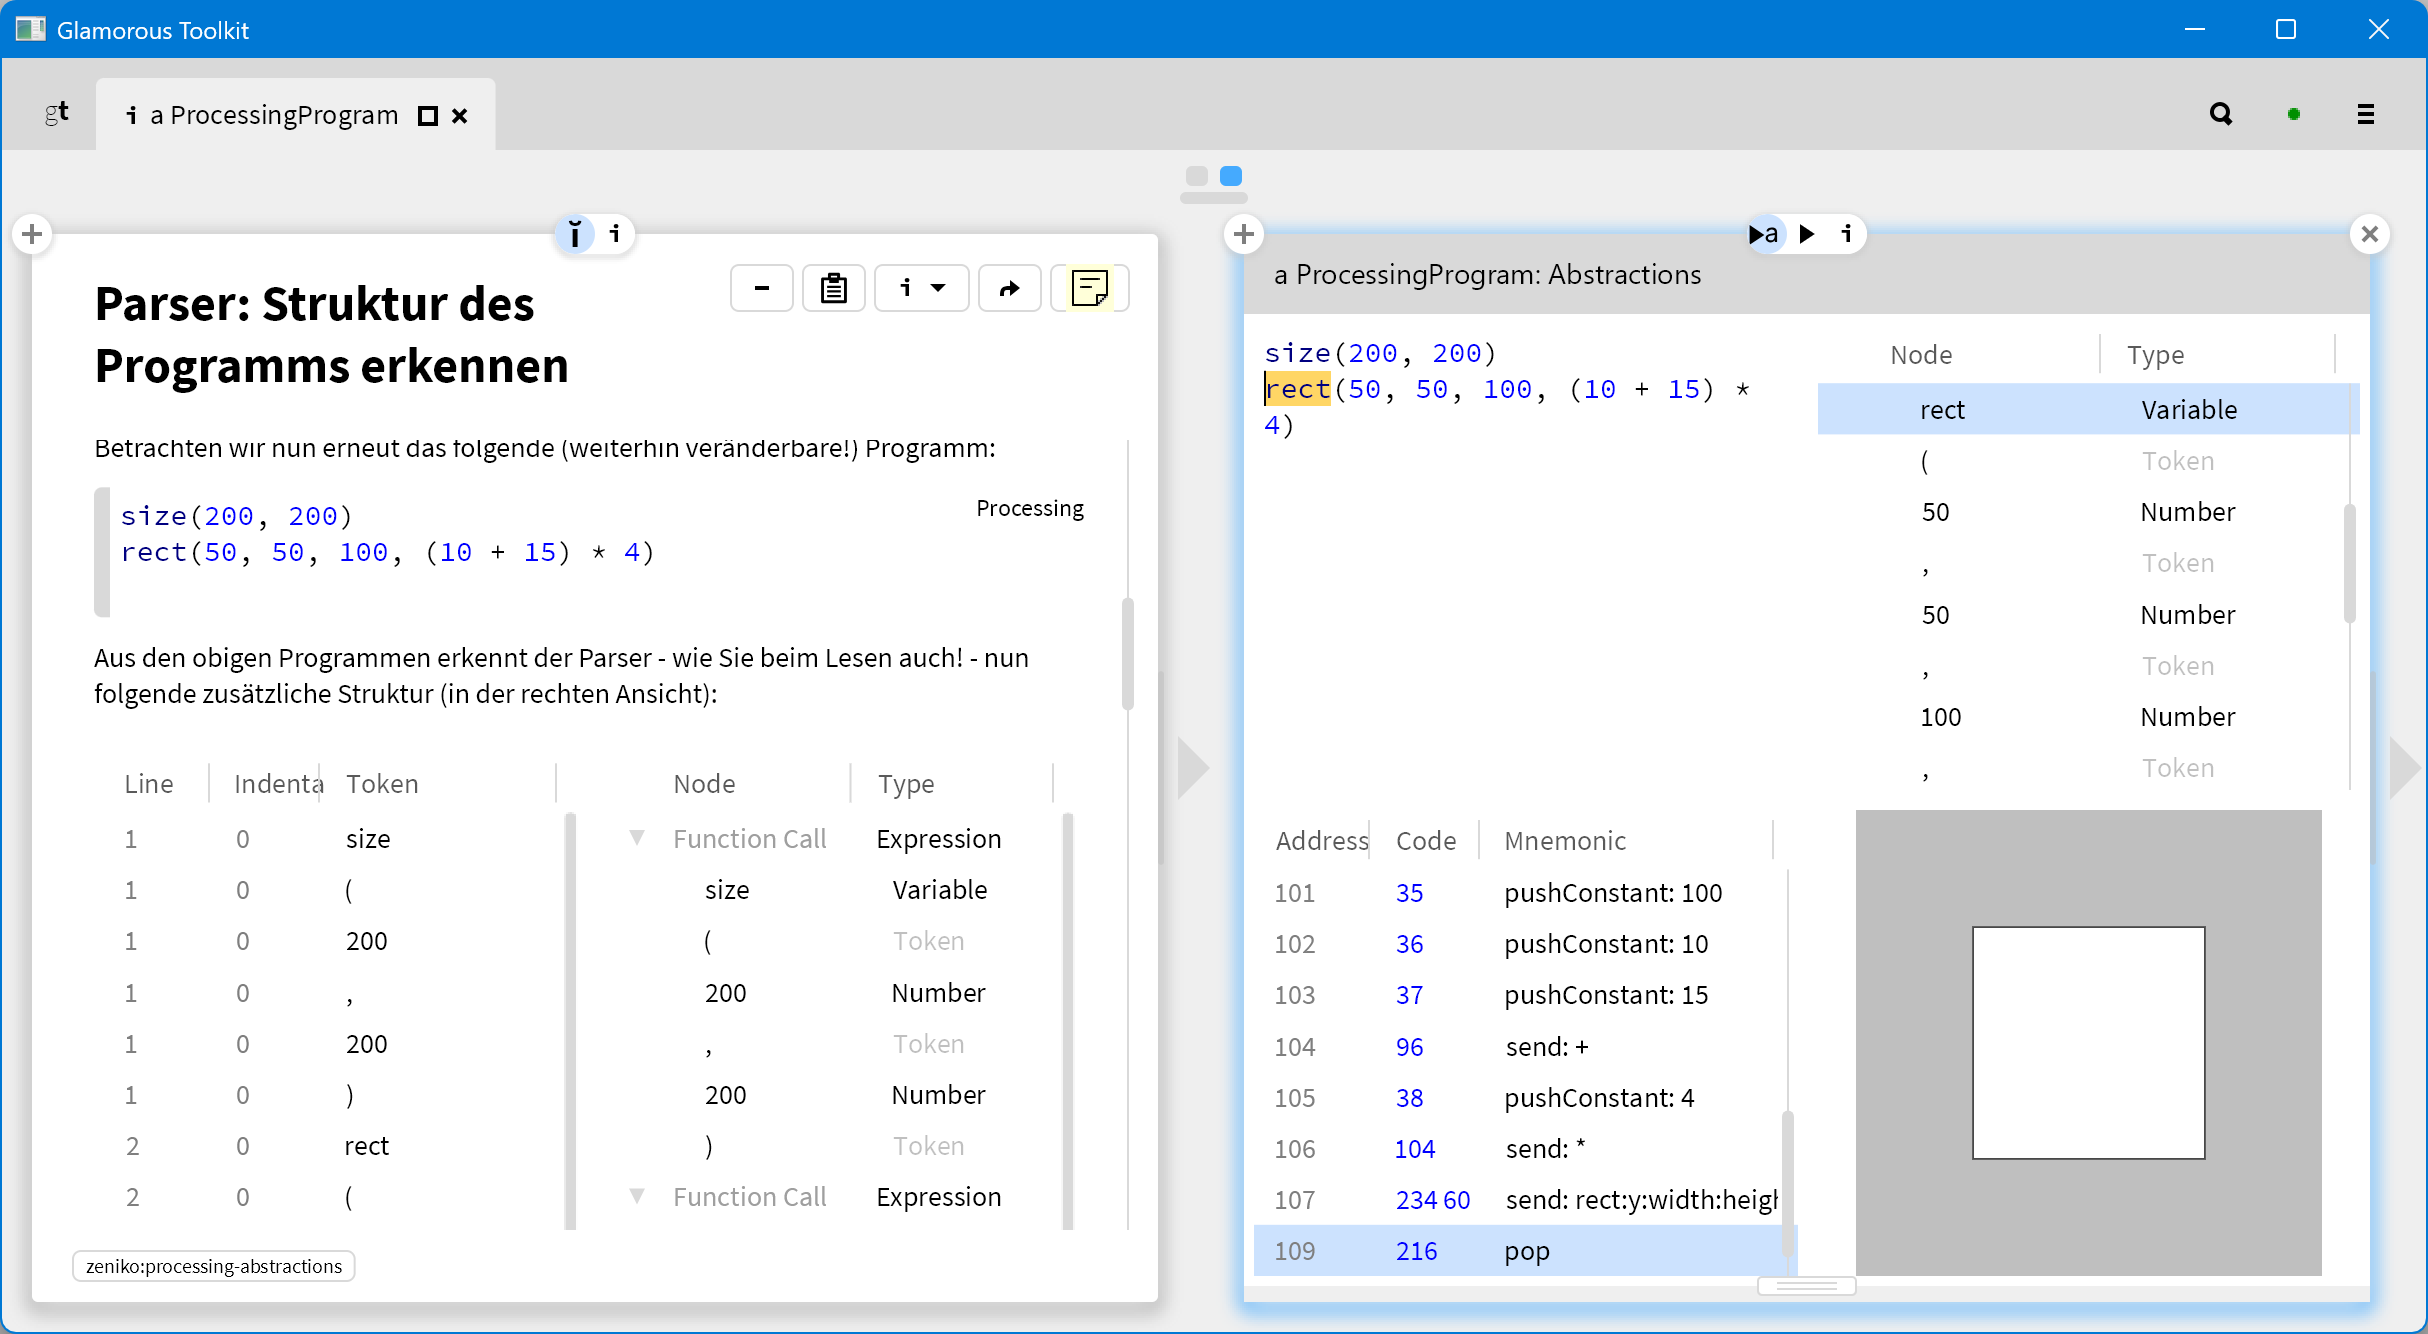
\includegraphics[width=.7\textwidth]{gt_screenshot}
\end{cfigure}

In its windows, \ac{GT} by default provides a tabbed interface which can show one of several tools: an object viewer, a notebook (dubbed ``Lepiter''), a code browser, a git interface and many more. While such tools are about as difficult to implement as an \ac{IDE} extension, the object viewer -- a tabbed interface itself -- is extended by simply annotating an object method which returns a \ct{GtPhlowView} object with the \ct{<gtView>} pragma as shown e.\,g. in figure \ref{fig_annotated_view}).

\begin{cfigure}[fig_annotated_view]{Smalltalk source required for creating a custom view.}
\begin{code}
ProcessingCodeBase >> gtOutputFor: aView [
	<gtView>
	^ aView explicit
		title: 'Output' translated;
		priority: 40;
		stencil: [ (ProcessingRunner new
				limitTo: (self gtIsAnimation ifTrue: [ 30 ] ifFalse: [ 2 ]) seconds;
				run: self clone;
				canvas) asElement ]
]
\end{code}
\end{cfigure}

In this example, the element passed to the \ct{stencil:} message -- here the canvas resulting from running a Processing program -- could instead also be displayed inside a notebook page, with no annotations needed at all. Annotations are thus only required to allow \ac{GT} to discover messages of a certain type.

Similarly, methods annotated with \ct{<gtExample>} are considered tests and can be collectively inspected and run for a class or an entire package. This achieves several goals of moldable development: What starts as throw-away code can be extracted into a method, annotated and remains then permanently available for repeated testing. Examples are also includable by name in notebooks, where they do function as (tested and thus guaranteed working) examples for documentation.

Since one of \ac{GT}'s stated goals is to make systems explainable \cite{Gir23}, it provides ample packages for loading, transforming and visualizing data in various forms such as the SmaCC parser generator\footnote{See \archivedurl{https://refactory.com/smacc/}.}, a graph builder \cite{Mey06}, \emph{etc.}, but also a built-in explanation system, allowing to visually connect arbitrary visual elements by annotating them (with a \ct{GtExplainerTargetAptitude} or a \ct{GtExplainerExplanationAttribute} respectively).

What might take some getting used to: All Smalltalk code and all live objects are stored in \ac{GT}'s \ct{.image} file which is updated whenever \ac{GT} is closed with saving. This means that there are no source files outside of \ac{GT}'s interface. Synchronization of Smalltalk code thus happens best through \ac{GT}'s built-in git client. Preexisting notebook pages are also stored within one of \ac{GT}'s subdirectories. Users can however create new pages in the ``Local knowledge base''\footnote{By default, this is located in the \ct{lepiter} subdirectory of the user's documents or home folder.} which can be backed up separatedly and which are stored even when \ac{GT} is quit without saving. All notebook pages indicate where they're stored in their footer and can be moved between databases through that footer. This allows students to take an existing page from teaching material and move it locally where it's separately backed up, in case they later delete or update \ac{GT}.


\subsection{Bleeding Edge Issues}

The developers of \ac{GT} follow a trunk-only development style without release branches. This means that the release version changes almost daily, with new features being introduced gradually. This also means that subtle issues might be unexpectedly introduced in a release by or as a side-effect of some partially implemented feature. As a consequence, if \ac{GT} with an app is to be distributed, the best way to do this is by downloading the latest version, loading the app into it, verifying that it works and then distributing \emph{this known good} image.

When \ac{GT} is used heavily, occasionally some lesser tested code paths might be hit. We've occasionally had some modifier keys apparently lock up, requiring app switching to get keyboard shortcuts working again; we've sometimes hit a cascade of error messages, spawning dozens of debug windows which had to be closed without other consequences; and occasionally \ac{GT} seemingly stopped responding, with even the \ct{Ctrl+.} keyboard shortcut not interrupting the running code (luckily, code modifications are backed up and restoreable through the ``Code changes'' tool). Most of these are small annoyances which more restrained users -- such as students -- shouldn't encounter often.

Finally, \ac{GT} is mainly developed under macOS and makes some platform assumptions with relation to its host operating system. This isn't noticeable when working purely within \ac{GT} but occasionally shows at its seams, with external executables not being located reliably for establishing a link to other runtimes\footnote{See GitHub issues \href{https://github.com/feenkcom/gtoolkit/issues/4608}{feenkcom/gtoolkit\#4608} for Linux and \href{https://github.com/feenkcom/gtoolkit/issues/4633}{feenkcom/gtoolkit\#4633} for Windows.}, knowledgebase names containing path separators\footnote{Which can be worked around by renaming the database, see GitHub issue \href{https://github.com/feenkcom/gtoolkit/issues/3036}{feenkcom/gtoolkit\#3036}.}, or pasting source code from third party apps leading to visual bugs in \ac{GT}'s code editor.\footnote{This applies under Windows, see GitHub issue \href{https://github.com/feenkcom/gtoolkit/issues/4634}{feenkcom/gtoolkit\#4634}.} We'd assume that most of the reported issues could have been fixed at the time of reading, though.


\subsection{Historical Remarks} \label{ssc_gt_history}

Smalltalk environments have been image-based and resumable since the early days in the 1970s, when Alan Kay sketched out the original Smalltalk which he eventually standardized at Xerox into Smalltalk-80. Based on a Smalltalk-80 \ac{VM} by Apple, Ingals, Kay \emph{et al.} started developing a new \ac{VM} and development environment which had the goal to also be customizable by non-programmers \cite{Ing97}: ``Squeak'' inherited its built-in capabilites for live and exploratory coding from the original Smalltalk and its back to this point that \ac{GT}'s heritage is tied directly.

While Squeak was further developed at Walt Disney Media Labs and among others included in the ``One Laptop per Child'' laptops, it remained a niche product -- likely due to missing interoperability between the live environment inside its \ac{VM} and outside code. Still, Squeak and its later fork Pharo continued being worked on and were actively being used in academia and related spin-offs. Eventually, a team around Tudor G�rba -- including this thesis' supporter Oscar Nierstrasz -- set out to implement their idea of a moldable environment on the basis of Pharo, thus creating \ac{GT} \cite{Fee25}. Version 1.0 has been released in 2023 and is still being actively worked on.

\ac{GT} thus has an illustrious lineage and has achieved support for many concepts asked for by literature: It's a moldable environment, supports a clean object-oriented language, allows for live and exploratory programming, still remains comparatively manageable and -- particularly relevant for this thesis -- allows for reflection at various levels, including for every object access to its method's source code, its compiled form and even its memory layout inside its \ac{VM}.

%%%%% The Solution %%%%%

\chapter{Proposed Solution: A New Teaching Environment for Programming} \label{ch_pa}

In order to let students have a \emph{Sichtenwechsel} with relation to programming, \ie have them experience several different abstraction layers involved between a program's source code and its execution, a new teaching environment dubbed ``Processing Abstractions'' is proposed:

Within \ac{GT}, we've implemented support for the Processing programming language and molded views for every implementation step along the way. This allows for creating interactive notebook pages containing source code and a variety of these views, showing \eg the \ac{AST} and resulting bytecode for the \ac{GT} \ac{VM} side-by-side.

In this chapter, we document the architecture of this environment and the reasons for the approaches chosen. If you want to inspect the environment yourself, see appendix \ref{app_setup} for how to install all referenced code\footnote{Remove the line \ct{GtExplorationHomeSection studentMode: true.} in order to also see our implementation notes.}



\section{Overview of ``Processing Abstractions''}

``Processing Abstractions'' consists of a transpiler for translating Processing source code into executable objects, a runtime environment, a large collections of views into various aspects of the program, and teaching materials using them.\footnote{The teaching materials currently provided are in the language used for teaching at the location of writing: German.} Tools and views as well as materials are all implemented within \acf{GT}, the former in Smalltalk code and the latter as ``Lepiter'' notebook pages.

\begin{cfigure}[fig_screenshot_vm_execution]{Excerpt from an interactive notebook page on program execution in a \ac{VM}.}
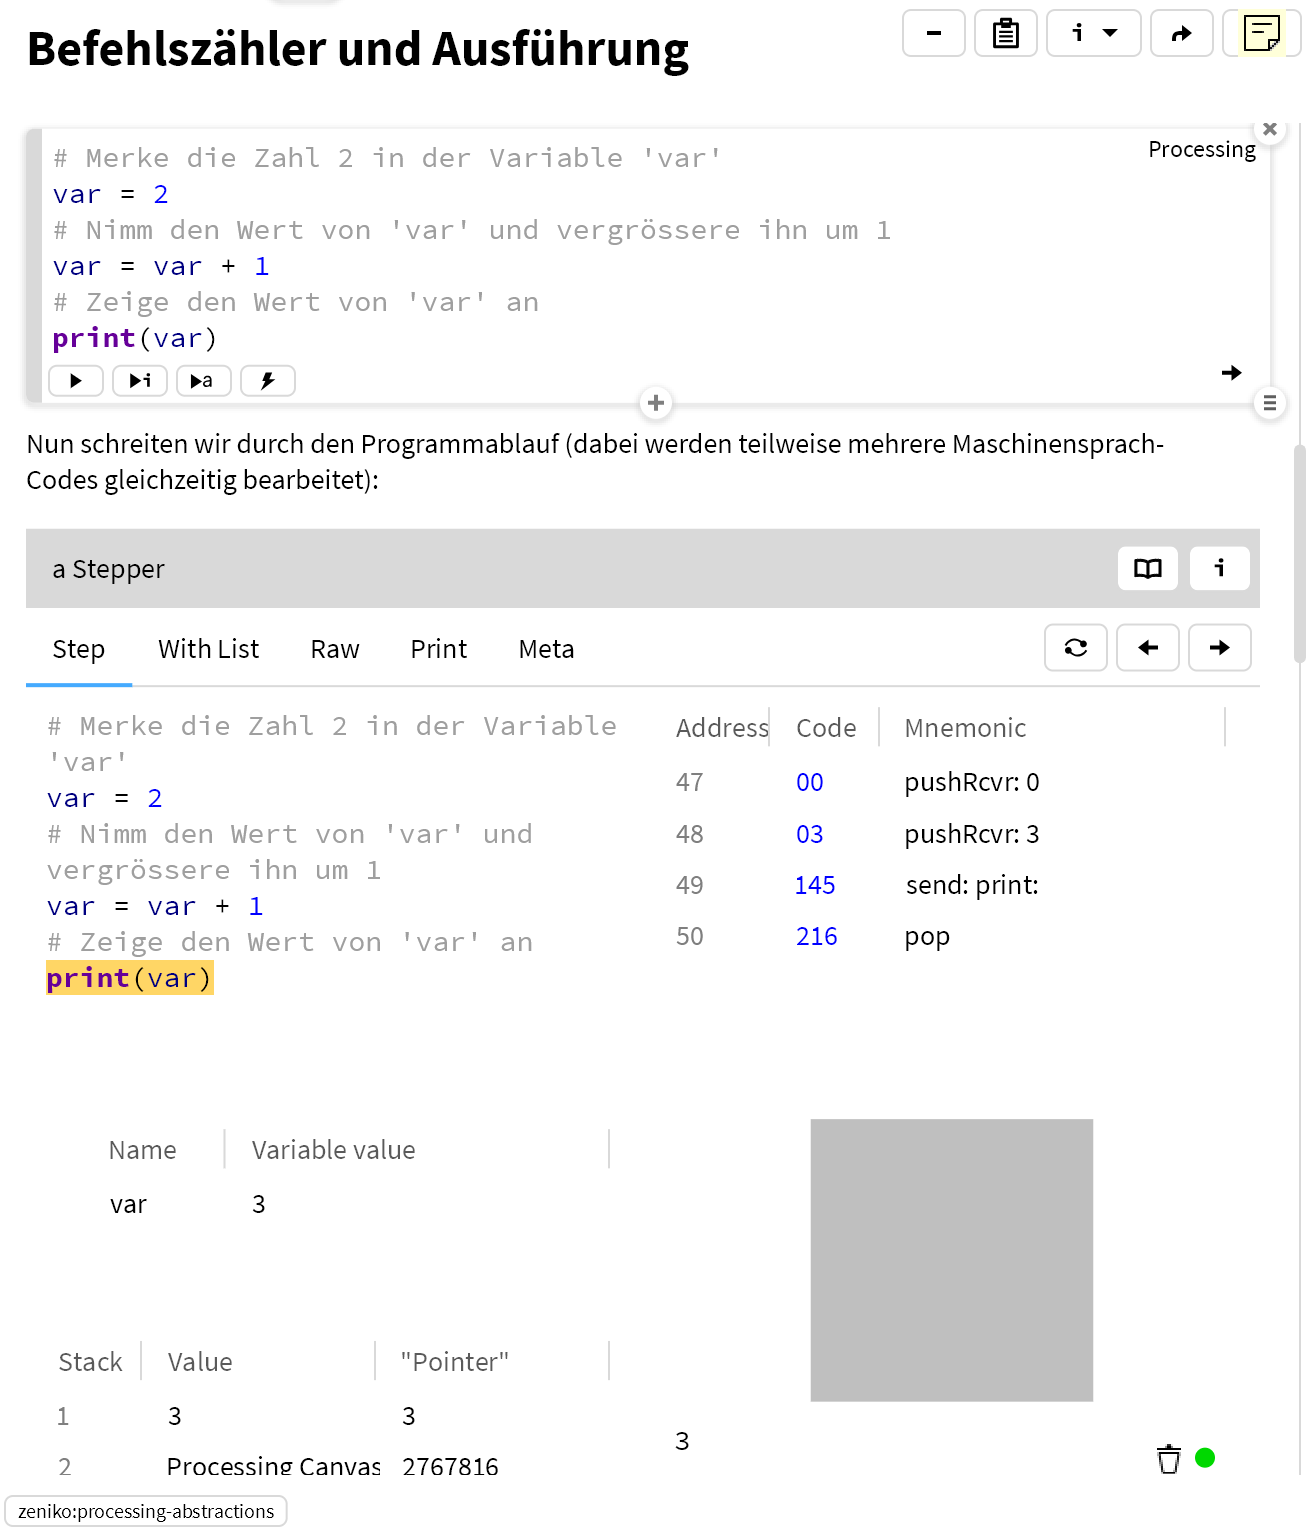
\includegraphics[width=.7\textwidth]{screenshot_vm_execution}
\end{cfigure}

Figure \ref{fig_screenshot_vm_execution} shows an excerpt from materials for students: The program visible at the top resides in a Processing-specific `snippet' with commands for running and inspecting the program independently of the page it resides on at the bottom; below a combined view for one execution step is shown with (clockwise) the step in question highlighted in source code; the corresponding bytecode visible; the program's output up to and including the current step; the contents of the execution stack of the Smalltalk \ac{VM}; and a list of all variable states.

Many such views are updated live whenever the source code is modified, without any other action required by students.\footnote{The one exception is the combined run-step view which for longer running programs would be too resource intensive to regenerate on the fly. Refreshing it manually is still possible.} The five views shown in figure \ref{fig_screenshot_vm_execution} can also be used on their own or in other arrangements (\eg only source and a full bytecode view where interacting with one automatically highlights the corresponding items in the other).

As will be shown below, dozens of premade views are available. Embedding any of them in a notebook page is done by adding an `Element' snippet with the one line of Smalltalk code shown in figure \ref{fig_embedding_view}. As an example, this code connects the first Processing snippet on the current page with a live \ct{gtTreePlusSourceFor:} view.

\begin{cfigure}[fig_embedding_view]{Smalltalk code for embedding a view in a notebook page}
\begin{code}
(ProcessingSource fromPage: thisSnippet page at: 1) renderLiveView: #gtTreePlusSourceFor:
\end{code}
\end{cfigure}

From these views, interactive teaching materials related to programming, compilers and code execution in a (virtual) machine can be composed, allowing students to combine their preexisting knowledge from programming with concepts of different abstraction layers.



\section{Exploring Abstraction Layers}

Any of the views into a program require its source written in Processing with Python syntax\footnote{Restricted to the implemented API as documented in appendix \ref{app_api}.} available either as a single file or as snippet in a \ac{GT} notebook. We recommend the latter, as views are then generally live and effects of changing the source code can be more easily explored by students.



\subsection{Source Snippet}

The ``Processing/Python'' snippet used in \ac{GT}'s notebook pages is the only place where Processing source code can be modified. It also provides several ways to run the program:

\begin{itemize}
\item {\small\faPlay} (or its shortcut \ct{Ctrl+R} for ``Run'') runs the program and either display its `Output' view or an inline error message.
\item {\small\faPlay}\texttt{i} (or its shortcut \ct{Ctrl+G} for ``debuG'') runs the program, recording all individual steps at the level of Python (sub)expressions -- allowing to step through the program's runtime views and inspecting among others the values of variables and the current state of the output.
\item {\small\faPlay}\texttt{a} (or its shortcut \ct{Ctrl+D} for ``Details'') shows the `Abstractions' view, \ie the program's main decomposition states: source code, \ac{AST}, bytecode, and output.
\item \lightning\ (or its shortcut \ct{Ctrl+Shift+D}) opens \ac{GT}'s Smalltalk debugger at the \ct{gtRun} entry point of the transpiled code for live debugging for either advanced students or for looking under the hood of the \ac{API} calls.
\end{itemize}

With just one source snippet, students can write and inspect programs with the opened views updating live as the program changes. This should give about the same experience as the Processing IDE with the main distinction that it's a live environment.

In contrast to the snippet, views are static in the sense that the source code can't be modified there.


\subsection{Output View}
% Source -> Output

The only views students should already know are the traditional `Source' and `Output' views which show the source code and the result of running the program respectively. Programs containing an animation loop will show the animation and allow user interaction in any output view.\footnote{Interactions are currently limited to mouse movements and clicks.}

The `Source' view is meant to be linked to any other view, allowing for interacting between them by selecting source expressions and having the corresponding item(s) in the other view(s) also selected.

The `Output' view can be used at any state to quickly verify visually that a program behaves as expected, be it during an introduction to programming or when exploring part of a program's execution or decomposition.\footnote{All of these views are directly available for a Processing program when running it using {\small\faPlay}\texttt{a} or \ct{Ctrl+D} and then selecting the \texttt{i} selector at the top (see figure \ref{fig_gt_screenshot} on page \pageref{fig_gt_screenshot}).}


\subsection{Compilation Views}
% Source -> Tokens -> AST -> Transpilation -> IR -> Bytecode

One way to show students what happens to a program before it can be executed on a (virtual) machine is to take them through the involved steps:

\begin{itemize}
\item The `Tokens` view (see figure \ref{fig_views_parser}) shows each of the tokens the lexer has encountered, including additionally required information such as a line number and line indentation\footnote{Indentation is relevant, as Python and as a consequence Processing with Python syntax is a language with significant whitespace, using common indentation for denotating code blocks.}. This view can be used for students to see what a compiler is looking at in their program with whitespace and comments in particular missing.\footnote{As a limitation, tokens are currently extracted in reverse from the parser which prevents inspecting tokens of syntactically invalid programs.}
\item The `\ac{AST}' view (see figure \ref{fig_views_parser}) shows the resulting parsing tree in a form that differentiates semantically relevant (sub)expressions from purely structural tokens. Combined with the `Tokens' view, this view can be used for hypothesizing and exploring how and what tokens are grouped together. In order to allow better interaction between `Tokens' and `\ac{AST}' views, the latter is a tree-list. A proper `\ac{AST} Tree' view is however also provided where the tree structure is more obviously visible, in particular also for larger programs.
\item The `Transpilation' view shows the result of translating the \ac{AST} to Smalltalk. Since the \ac{AST} needs to be barely modified for this translation step, Smalltalk code should be relatively easy to understand, at least when the original Processing source is displayed in parallel.

The `Transpilation' view also allows students to see what Processing does implicitly behind the scenes: setting and updating implicit variables, such as \ct{width}, \ct{mousePressed}, \etc, calling \ct{setup} once and \ct{draw} repeatedly, and running top-level code before entering the animation loop (see figure \ref{fig_animation_loop}).

In order to discuss programming language syntax, two additional views `Prefix' and `Postfix' show transpilations into a Lisp-like language using S-expressions and a Postscript-like language with reverse polish notation respectively. These may also serve as a basis for students' own parser projects, translating these pseudo-languages back into Processing or Smalltalk.
\item The `\acs{IR}' view shows the \ac{IR} generated by the Smalltalk Opal compiler from the transpiled Smalltalk code. With variable names still showing and optimizations still missing, this allows students to make more sense of the eventual bytecode, in particular when both views are displayed side-by-side.
\item The `Bytecode' view finally shows the bytecode which will be run by the Smalltalk \ac{VM}\footnote{Unless it's later translated to native code by the \ac{JIT}.} with instruction addresses\footnote{These are actually byte indices in the method's binary layout as used by the Smalltalk \ac{VM}.} and mnemonic added so that jumps can be understood and the code can be more easily connected to either \ac{IR} or any other form of Assembly language.
\end{itemize}

All of these views can be linked together, so that selecting an item in one view will highlight the corresponding item(s) in the linked views. The default `Abstractions' view, available directly from every Processing snippet, \eg combines the source with `\ac{AST}', `Bytecode' and `Output' (visible on the right hand side in figure \ref{fig_gt_screenshot} on page \pageref{fig_gt_screenshot}, with a source expression and its corresponding items highlighted).

\begin{cfigure}[fig_views_parser]{Screenshot of a page of student content showing modifyable Processing source with live views for tokenization (left) and abstract syntax tree (right).}
\centering
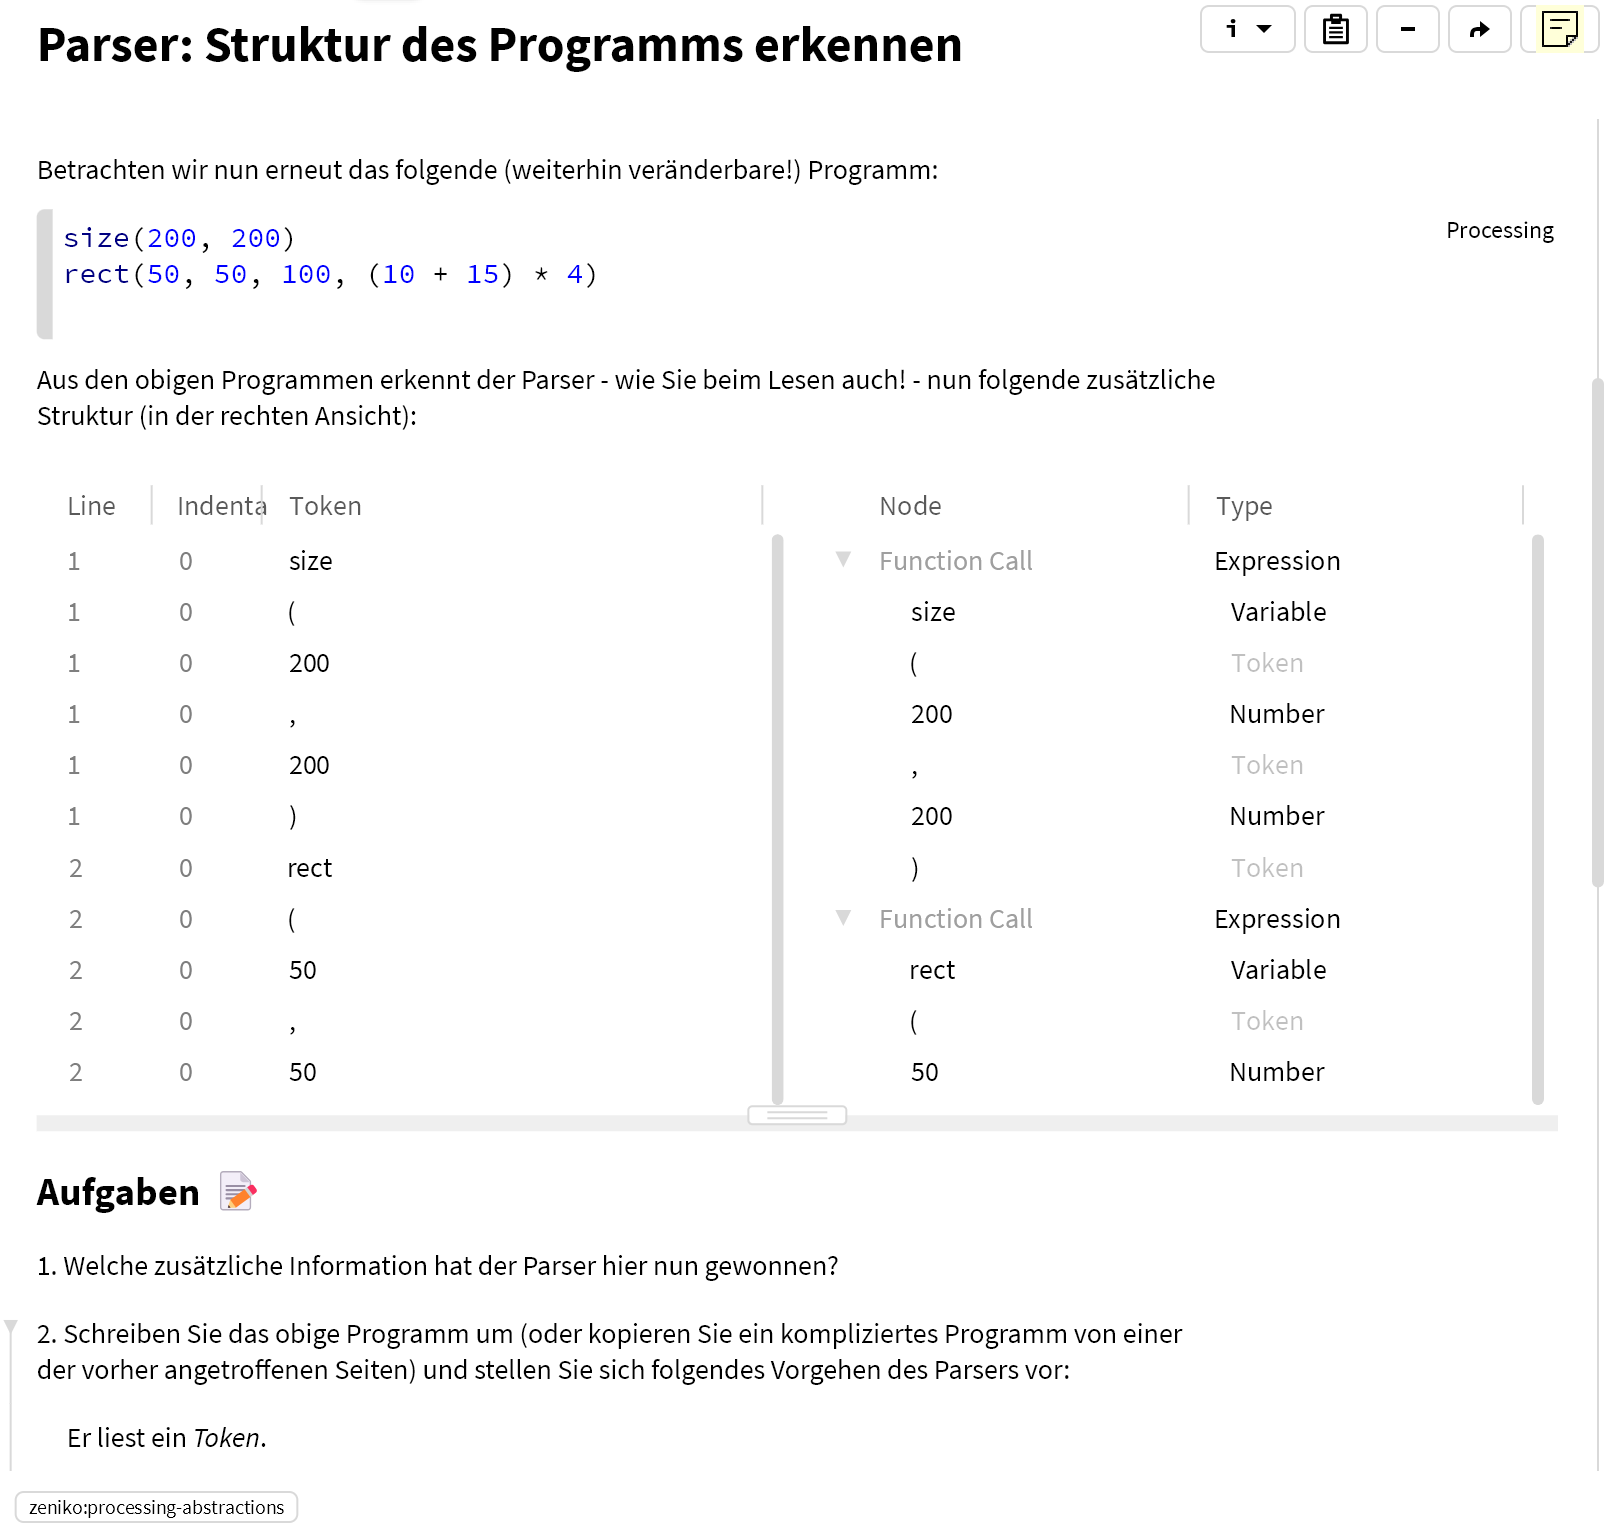
\includegraphics[width=.8\textwidth]{screenshot_parser}
\end{cfigure}

\begin{cfigure}[fig_animation_loop]{Implicit animation loop (Transpilation view) and part of the required \ac{API} (only visible when debugging transpiled code)}
\begin{code}
SubclassOfProcessingCodeBase >> gtRun
	self setup.
	[ gtCanvas frameRate > 0 ] whileTrue: [
		mouseX := gtCanvas mouseX. mouseY := gtCanvas mouseY.
		mousePressed := gtCanvas mousePressed.
		self draw.
		gtCanvas endFrame.
	].
\end{code}

\begin{code}
ProcessingCanvas >> endFrame [
	presenter updateOutput.
	(1 / frameRate) seconds wait.	"The frame rate is adjustable through `frameRate()`"
	frameCount := frameCount + 1.
	transform := #yourself	"Transforms are reset at the end of a draw-cycle"
]
\end{code}
\end{cfigure}


\subsection{Run Step Views}
% Run Step -> Source -> Bytecode -> Execution Stack -> Variables


Finally, there's three views tied to a program's runtime which may be helpful even for a pure introduction to programming: \ct{gtOutptFor:} shows the output of a program which may continuously change, if the program describes an animation, and which may be interacted with\footnote{For now only using the mouse which changes the implicit variables \ct{mouseX}, \ct{mouseY} and \ct{mousePressed} and calls the callbacks \ct{mousePressed}, \ct{mouseReleased}, \ct{mouseClicked} and \ct{mouseMoved} if any of them has been defined by the user.}; \ct{gtOutputShapesFor:} allows inspecting the individual shapes in the order they've been rendered (this view is disabled for animations); and \ct{gtStepsFor:} shows an overview of all views of \ct{ProcessingRunStep} for every Processing (sub)expression that has been evaluated -- including the expression in the source, the transpilation and its bytecode form, current variable values, values on the Smalltalk \ac{VM}'s stack and the current output state. This gives us a debugging view in which a student can step forward and backward through the execution of the program but also shows an excerpt of the different layers involved in program execution.


\subsection{Source Data}
% Source -> Characters -> Bytes

At the level of source code, there's three different views showing the source with syntax highlighting (\ct{gtContentsFor:}), showing the individual source characters with their unicode value (\ct{gtSourceCharsFor:}), and showing the bytes as they would be written to disk, assuming the default UTF-8 encoding also used by the original Processing \ac{IDE}, with bytes also displayed in hexadecimal and binary notations (\ct{gtSourceBytesFor:}). With these views and suitable sample code, students might be able to deduce some regularities with relation to ASCII character ranges and UTF-8 encoding.


\subsection{Other Views}
% Source -> Slices
% Source -> Shapes



\section{Implementation Details}


\subsection{Views}

All views in \ac{GT} are by convention provided by methods with names of the form \ct{gt...For:} and are categorized as ``views'' in the class browser.\footnote{Actual requirement is only the \ct{<gtView>} pragma annotation and the method signature (\ct{GtPhlowView} $\rightarrow$ \ct{GtPhlowView}).}

With any view visible in \ac{GT}, \ct{Alt}+clicking on a view's name shows its source method(s), revealing the view's method name and implementation. The method name will be required for embedding a view in a notebook page as described in figure \ref{fig_embedding_view} above.

For comparing the same views of different programs, the \ct{ViewComparison} helper class is provided which can be used in `Element' snippets as follows:

\begin{code}
ViewComparison newFor: {
	(ProcessingSource fromPage: thisSnippet page at: 1) program -> #gtSourceCharsFor:.
	(ProcessingSource fromPage: thisSnippet page at: 2) program -> #gtSourceCharsFor:.
}
\end{code}


Any of these views can be integrated on its own into an interactive notebook page for producing student content, they are however also all available to students through the Processing/Python snippet's various execution modes: Either running the program for pure output ({\small\faPlay} or \ct{Ctrl+R}) gives access to the most common views by inspecting the object behind the output ({\small\faPlay}\texttt{i} in the upper right corner); or running the program for details ({\small\faPlay}\texttt{a} or \ct{Ctrl+D}) yields all the views through \texttt{i} at the top center. For manageability, both of these options can be ignored at the start, as the default views should provide sufficient informations and the remaining ones can be continually introduced during class.


\section{Classes}

%%%%% The Solution (UML Diagram) %%%%%

\newgeometry{bottom=1cm}

\begin{landscape}

\begin{cfigure}[fig_uml_processing]{Diagram of most classes involved in running Processing code within \ac{GT}}

\begin{tikzpicture}

\begin{package}{Processing}

\begin{class}[text width=6cm]{ProcessingSource}{0, 0}
\operation{fromFile:}
\operation{fromPage:at:}
\operation{fromSnippet:}
\end{class}

\begin{class}[text width=6cm]{ProcessingProgram}{0, 2.5}
\operation{ast}
\operation{compilation}
\operation{run}
\end{class}

\begin{class}[text width=6cm]{ProcessingParser}{-8, 0}
\operation{parse:}
\end{class}

\begin{class}[text width=6cm]{ProcessingTranspiler}{-8, 2.5}
\operation{transpile:}
\end{class}

\begin{class}[text width=6cm]{ProcessingTranspilationSlice}{-8, 7.5}
\operation{link:method:from:to:}
\end{class}

\begin{interface}[text width=6cm]{ProcessingCodeBase}{0, 5}
\operation{gtRun}
\end{interface}

\begin{class}[text width=6cm]{ProcessingRunner}{8, 5}
\operation{run:}
\operation{runSteps:}
\end{class}

\begin{class}[text width=6cm]{ProcessingCanvas}{0, 7.5}
\operation{asElement}
\operation{presenter}
\end{class}

\begin{class}[text width=6cm]{ProcessingCanvasPresenter}{8, 7.5}
\implement{ProcessingCanvas}
\end{class}

\begin{class}[text width=6cm]{ProcessingCanvasElement}{8, 9}
\end{class}

\begin{class}[text width=6cm]{ProcessingAstCleaner}{-8, 5}
\operation{clean:}
\end{class}

\begin{interface}[text width=6cm]{ProcessingCanvasShape}{0, 9}
\end{interface}

\begin{class}[text width=6cm]{ProcessingRunStep}{8, 2.5}
\end{class}

\draw[umlcd style dashed line, ->] (ProcessingSource) -- node[black]{$<<$accesses$>>$} (ProcessingProgram);
\draw[umlcd style dashed line, <->] (ProcessingProgram) -- node[black, sloped]{$<<$source $\rightarrow$ \ac{AST}$>>$} (ProcessingParser);
\draw[umlcd style dashed line, ->] (ProcessingProgram) -- node[black]{$<<$uses$>>$} (ProcessingTranspiler);
\draw[umlcd style dashed line, ->] (ProcessingTranspiler) -- node[black, sloped]{$<<$creates$>>$} (ProcessingCodeBase);
\draw[umlcd style dashed line, <->] (ProcessingTranspiler) -- node[black]{$<<$uses$>>$} (ProcessingAstCleaner);
\draw[umlcd style dashed line, ->] (ProcessingTranspiler.west) -- +(-1, 0) |- node[black, pos=0.25, sloped]{$<<$creates$>>$} (ProcessingTranspilationSlice);
\draw[umlcd style dashed line, ->] (ProcessingProgram) -- node[black]{$<<$accesses$>>$} (ProcessingCodeBase);
\draw[umlcd style dashed line, ->] (ProcessingProgram) -- node[black, sloped]{$<<$uses$>>$} (ProcessingRunner);
\draw[umlcd style dashed line, ->] (ProcessingRunner) -- node[black]{$<<$runs$>>$} (ProcessingCodeBase);
\draw[umlcd style dashed line, ->] (ProcessingRunner) -- node[black]{$<<$creates$>>$} (ProcessingRunStep);
\draw[umlcd style dashed line, ->] (ProcessingCodeBase) -- node[black]{$<<$owns$>>$} (ProcessingCanvas);
\draw[umlcd style dashed line, ->] (ProcessingRunner) -- node[black, sloped]{$<<$creates$>>$} (ProcessingCanvas);
\draw[umlcd style dashed line, ->] (ProcessingCanvas) -- node[black]{$<<$controls$>>$} (ProcessingCanvasPresenter);
\draw[umlcd style dashed line, ->] (ProcessingCanvasPresenter) -- node[black]{$<<$interacts$>>$} (ProcessingCanvasElement);
\draw[umlcd style dashed line, ->] (ProcessingCanvas) -- node[black]{$<<$creates$>>$} (ProcessingCanvasShape);
\draw[umlcd style dashed line, ->] (ProcessingCanvasShape) -- node[black]{$<<$renders$>>$} (ProcessingCanvasElement);

\end{package}

\end{tikzpicture}

\end{cfigure}

\end{landscape}

\restoregeometry


\ac{GT} was chosen for its moldable environment: As shown in \ref{sc_gt}, different views are quick to implement and can be combined freely with interactions and updates between them.

Since \ac{GT} is based on Smalltalk, an initial effort is required to learn language and environment before these benefits can be used. This is helped by Smalltalk's regular syntax and \ac{GT}'s reflective capabilities.\footnote{For Smalltalk and \ac{GT}'s ancestor Pharo, there are sufficient resources available online, for \ac{GT} itself, there's the ``Glamorous Toolkit Book'' \cite{Gir23} and a Discord server.}

Implementing a new language in \ac{GT} can happen along the moldable patterns documented in \ref{sc_moldable}: Starting with concrete samples, classes and views for handling them are molded in steps until the desired behavior is reached; then code is refactored into permanent methods on the one hand and a concrete example serving as test case on the other. Whenever the need for a different view into the program or one of its intermediary forms (such as \ac{AST}, bytecode or output) arises, the view is constructed in the same way by first iteratively shaping the data into the desired form and then either passing this to one of \ac{GT}'s standard views (text, list, tree, table, forward) or composing the view's layout in the same way iteratively.

The product consists of the following main classes which can be found in \ac{GT} through the spotter (\faSearch):

\ct{ProcessingCanvas} provides the implementation of most of the Processing \ac{API} for rendering the various shapes in the form of \ct{BlElement}s (wrapped through \ct{ProcessingCanvasShape}). It does this through \ct{ProcessingCanvasPresenter} into a \ct{ProcessingCanvasElement} of which there can be multiple, allowing to use a canvas for multiple views. The canvas also provides access to the individual shapes and all of its state. Rendering onto the canvas happens through the transpiled and compiled Processing program for which a new canvas is created for every separate run.

Processing programs can be written either inside \ac{GT}'s notebook in form of a ``Processing/Python'' snippet, in form of a Smalltalk string or in separate files. All forms are loaded through the \ct{ProcessingSource} class. Since we mostly want Processing source and its various views to be seen in a notebook page, the most common way to process a Processing program will be inside the page through\footnote{The \ct{at: 1} part of the message may also be omitted, if there's only one snippet on a notebook page. Omit the \ct{renderLive} message, if you want access to any of the intermediary states or different views.}
\begin{code}
(ProcessingSource fromPage: thisSnippet page at: 1) renderLive
\end{code}




The snippet is implemented in \ct{LeProcessingSnippet} which builds upon \ac{GT}'s \ct{LePythonSnippet} for syntax highlighting but accesses Processing through \ct{ProcessingSource} instead of Python through \ct{PythonBridge}.

For embedding output or any other view inside a notebook page, an ``Element'' is added with either the code from above or with \ct{renderLive} replaced with \ct{renderLiveView:} with the symbol of the desired view appended (\ct{#gtTreeFor:}, \ct{#gtTranspilationFor:}, \ct{#gtBytecodeFor:}, \etc; see the ``views'' category of \ct{ProcessingSource} and \ct{ProcessingProgram} for all available views).

For all the views, a \ct{ProcessingProgram} is created through \ct{ProcessingSource>>>program} which transforms it into its various forms:

\begin{itemize}
\item \ct{ProcessingParser} is used for parsing the source into an \ac{AST}. Since Processing shares Python's syntax, the parser is a very thin wrapper around \ac{GT}'s \ct{PythonParser}. The \ac{AST} is then slightly modified through \ct{ProcessingAstCleaner} to better map Python to Smalltalk: Since statements after a \ct{return} are allowed in Python but not supported in Smalltalk, they're silently dropped (a warning about unreachable code could be added); and parenthesized expressions are parsed into \ct{PyTupleExpressionNode} which complicate later optimizations with relation to operator chains, in particular logical operators \ct{and} and \ct{or}.
\item \ct{ProcessingTranspiler} then walks through the cleaned \ac{AST} and transpiles Python expressions to the corresponding Smalltalk, recording a \ct{ProcessingTranspilationSlice} for every (sub)expression, thus later allowing to map bytecode its mapping into Smalltalk code back to the corresponding Processing source. If \ct{setup} and/or \ct{draw} functions are defined in Processing code, the implicit animation loop is added to the end of top-level code. Processing \ac{API} calls -- if not overwritten by user code -- are translated through messages of the form \ct{ProcessingTranspiler>>>emit_...:} which the transpiler detects through reflection.
\item The transpiled code is compiled to methods of an anonymous subclass of \ct{ProcessingCodeBase}. This base class provides views at the lower abstraction levels from transpiled code to bytecode and also the entry point to the user supplied program \ct{gtRun} which contains top-level code. Global variables are turned into instance variables, thus being available to all Processing functions in the form of Smalltalk methods.\footnote{In order to prevent overriding of \ct{gtRun} and the different view messages, Processing names starting with \ct{gt} are renamed to starting with \ct{gt_} during transpilation.}
\end{itemize}

While compiled Processing programs can be run directly, \ct{ProcessingRunner} is used for ensuring the presence of an output canvas, for allowing program execution to be interrupted and for extracting \ct{ProcessingRunStep} instances for every Processing (sub)expression.

From these, \ct{ProcessingProgram} provides all views corresponding to Processing code and combined views. In order not to overwhelm students with too many views, \ct{gtDefaultInspectorTool} has been implemented for hiding all but the main four views behind the same symbols as used by the snippet.

During compilation, most common exceptions are \ct{SmaCCParserError} during parsing, \ct{ProcessingCompileTimeException} during transpilation and \ct{ProcessingRunTimeException} during execution. At this point, exceptions occurring in the transpiled code are not translated yet. Since most programs are meant to be re-run live, a heuristic has been implemented for catching endless loops which may naturally occur while a program's source is modified where \eg a variable's value is modified but at the end of a \ct{while} loop. Instead of detecting the endless loop from code, runtime has been restricted to a maximum of two seconds for non-animated programs and thirty seconds for animated programs.



\section{Usage}

With this, high school teachers get a toolkit for teaching programming and systems at various levels:

At the start of a course, the environment can be used as an introduction to programming (see the suggested lessons in \ref{sc_lesson_intro}). When the limitations of the environment are reached, the move over to the official Processing \ac{IDE} should be seamless: code copied over and run (with the same icon and shortcut) yields the same output and can then be further modified with the full Processing \ac{API}, once students are ready.

When teaching computer architecture, the environment can be used for either exploring the various abstraction levels involved or even again as a full course embedded in notebook pages (see \ref{sc_lesson_ca}). In case of both usages, this better ties together programming and system architecture. And if programming has happened in Processing, students can investigate their own programs instead of mainly relying on those given by the teacher.

In an in-depth course for students specializing in computer science, this environment can further be used to teach the inner workings of a compiler from lexer to optimizer (see \ref{sc_lesson_compiler}).

Finally, this environment could also be used as a stepping stone for introducing Smalltalk as a different programming language and \ac{GT} as the moldable environment it is, leading students to molding the provided materials further by \eg extending the Processing \ac{API}, developing new views or starting to work on a language of their own (see \ref{sc_lesson_other}).

In all cases, \ac{GT} can also be used as a digital notebook by students, where they solve tasks directly in the page, add their own notes and keep their modified examples.

While this environment is mainly targetted at high school students, it could also be used in middle school. For middle schoolers, the exposed user interface would however have to be reduced as far as possible to keep it manageable. It could however work at least in a smaller group with interested and motivated students wanting to step beyond block based programming languages. For university students, there's currently not enough depth available.


\section{Other approaches considered}

A stable snapshot of the code discussed here is available at \url{https://github.com/zeniko/gt-exploration/tree/thesis}.

Within \ac{GT}, Processing is implemented through transpilation to Smalltalk. This allows reusing several of \ac{GT}'s libraries: \ct{PythonParser} for parsing Processing with Python syntax and \ct{OpalCompiler} for compiling Smalltalk with bytecode extractable through \ct{CompiledCode>>>symbolicBytecodes}.

Since Processing implemented on top of Python is a strongly but dynamically typed language, it maps well onto Smalltalk which is the same. Still, initially three other approaches were considered:

Processing could be run either in the original \ac{JVM} and then accessed through Python or directly run using one of several Python libraries \cite{Tab22}. In all cases, its objects would be accessed through \ct{PythonBridge}. Since at the time of writing, support for PythonBridge under Windows was difficult to achieve in a portable manner (\ie without requiring students to install multiple different packages which increases the risk of accidental breaking and thus potential support issues), this approach was rejected.

Alternatively, Processing could have been implemented through an interpreter in \ac{GT}\footnote{Remnants of which are available as \ct{ProcessingInterpreter}.}. This would have required to write a separate compiler for creating bytecode just for demonstration purposes. Instead, a compiler from Processing to Smalltalk bytecode could have been written.\footnote{A compiler for a tiny subset of Processing is included as \ct{ProcessingCompiler}.} While this would have allowed for closer control over optimizations, it would effectively have become a reimplementation of most of \ct{OpalCompiler}.



\section{Potential Drawbacks}

While Modrow and Strecker prefer a block based language, we feel that at least parts of their issue with a text based programming language can be remedied by having a live environment with custom error messages. For remedying their remaining issue about allowing individual bits of code to be called independently, that could be achieved in one of the ways \ac{GT} does this: either by offering separate playgrounds which do work similarly to a \ac{REPL}; by allowing multiple code snippets to access the same environment (as it also works in Jupyter notebooks); or by allowing only selected code to be executed. The last option would be easiest to implement.\footnote{It hasn't been implemented for three reasons: At least in the beginning, it might confuse students more than it helps, which goes against manageability (see \ref{ssc_manageability}); most visual commands can't be executed entirely independently in Processing, as output always depends on \ct{size} and maybe other stateful commands; and interaction with the animation loop would have to be figured out: whether it's has to be paused during the entire interaction, just between two user commands or even not at all.}

Chiodini \etal \cite{Chi23} also propose starting with visual programming but have different requirements: In order to keep an introductionary language manageable, they ask among others for a limited \ac{API} which should be expandable by students (see also \ref{ssc_manageability}). And the full Processing \ac{API} can indeed be quite overwhelming, so only a subset must be introduced at the start. Indeed also for this reason only a subset has been implemented in \ac{GT} (see appendix \ref{app_api}), although already including some seemingly unnecessary functions: \eg the \ct{circle} function is easily implemented in terms of the more generic \ct{ellipse} function (see figure \ref{fig_circle}) -- either in the implementation of the Processing \ac{API} or by students.

\begin{cfigure}[fig_circle]{Implementation of \ct{circle} as built-in \ac{API} and in user code}
\begin{minipage}{.5\textwidth}
\begin{code}
ProcessingCanvas >> circle: x y: y d: d
	self
		ellipse: d
		by: d
		at: x @ y
\end{code}
\end{minipage}
\begin{minipage}{.45\textwidth}
\begin{code}
def circle(x, y, d):
	ellipse(x, y, d, d)
\end{code}
\end{minipage}
\end{cfigure}

Another requirement by Chiodini \etal is for problems to be transparently decomposed and solutions recomposed. This is indeed an issue with Processing: Moving a composed shape to a different location requires adjusting the coordinates of all basic shapes involved, therefore variables and even functions have to be introduced sooner rather than latter to allow the examples shown \cite{Chi23} to work. Similar to how they introduce a library to achieve their desired \ac{API}, the same functionality could be implemented on top of Processing at a later stage if desired.\footnote{In the provided teaching materials, an example of how to implement a simpler Turtle based \ac{API} is provided (see ``Schildkr�ten und Rekursion'').}

The main reason for not introducing a new \ac{API} as proposed by Chiodini \etal is the same as the reason for not introducing an entirely new programming language optimized for teaching (as done \eg by Black and Bruce \cite{Bla18}): This prevents benefiting from the large community and preexisting documentation and example code.

\begin{todo}
\item Shorten ``Implemented Classes'', move the details into an appendix
\item Decide which screenshots belong into the appendix instead.
\item use 2DET taxonomy? \cite{Sor13}
\end{todo}

%%MAIN: thesis.tex

%%%%% The Validation %%%%%
\chapter{Implementation: Lesson Plans} \label{ch_teaching}
% formerly: Teaching with \texttt{PA}
In its current form, \texttt{Processing Abstractions} as presented in chapter \ref{ch_pa} is mainly targetted at the obligatory introduction to computer sciences at high school level.

Before going into empirical results from using \texttt{PA} in two courses, three lesson plans will be presented for which \texttt{PA} has been developed: a \emph{Sichtenwechsel} in computer architecture (section \ref{sc_lesson_ca}); an introduction into the inner workings of a compiler (section \ref{sc_lesson_compiler}); and a plan for a general introduction to programming (section \ref{sc_lesson_intro}). Some ideas for how to expand it for other school levels will be presented in section \ref{sc_lesson_other}.

For all the lessons, students will need a local environment of \texttt{Processing Abstractions} installed on a computer available to them. See appendix \ref{ch_setup} for how to set it up. Additionally, for non-German speaking students the contents will have to be translated to the teaching language.

\section{Introduction to Programming} \label{sc_lesson_intro}
Using PA as a live programming environment.

\subsection{Educational objective}

\begin{todo}
\item students are able to write programs producing given outputs
\item students are able to read and understand programs with a limited, given command set
\item students learn from their mistakes, correct themselves, aren't afraid to break things
\item students have a solid foundation for taking on a task of writing a basic but still interesting app/game
\end{todo}

\subsection{Prerequisites}

Just the basics:
\begin{todo}
\item using own computer
\item downloading and installing, handling (ZIP) archives and virus scanners (under Windows at least)
\item curiosity, ...
\end{todo}

\subsection{Introduction to Glamorous Toolkit} \label{ssc_lesson_gt}

\begin{todo}
\item Distribute GT/PA
\item After extracting GT, a brief overview is needed before starting
\item Introduction to GT as an interactive notebook (compare to previously known software such as OneNote or Jupyter)
\item GT is bleeding edge (development on trunk), introduce most pressing issues (navigation, keyboard issues, saving, scrolling, zooming)
\item Some quick tasks for getting the hang of it and identifying students with more supporting needs (let them help themselves)
\item Point more advanced students towards inspectability
\end{todo}

\subsection{Lesson Plans}

\begin{todo}
\item stepwise introduction to Processing (introduced in \ref{sc_processing})
\item imperative, few commands: \texttt{size}, \texttt{rect}, \texttt{ellipse}, \texttt{fill}
\item teaches importance of order
\item tasks: produce given output
\item debugging consists in modifying values (result is immediately visible)
\item quicker and more proficient students can easily skip ahead (loops, animations, recursion)
\item introduce variables, loops, animation, interaction
\item available tools: output, step-by-step debugger (for now, more later)
\end{todo}


\section{Lesson on Compilers} \label{sc_lesson_compiler}
Using PA to demonstrated the steps of lexing, parsing, transpiling, compiling and optimizing.

Part of this has been validated (cf. \ref{sc_validation_compiler})

\subsection{Educational objective}

\begin{todo}
\item students can explain the difference between high and low level language
\item students can enumerate the steps required for compiling a program
\item students have an understanding of the roles a lexer, parser, transpiler and compiler play
\end{todo}


\subsection{Prerequisites}

\begin{todo}
\item programming with Processing (e.g. from \ref{sc_lesson_intro})
\item GT/PA installed (e.g. from \ref{ssc_lesson_gt})
\item Stacks and registers
\end{todo}


\subsection{Lesson Plan}

\begin{todo}
\item Repetition high level programming (see tasks in PA)
\item Comparision with low level programming (e.g. \cite{Tom15}): levels 1 to 6 (introduces jumps, memory access, arithmetic)
\item Presenting/reading overview, compare with natural language
\item Lexer: compare given example with mainly different whitespace; what are tokens?
\item Parser: describe AST in own words, compare with sentence structure from natural languages; develop simple parsing model (\xxx{better views?})
\item Transpiler (optional): compare Processing and Smalltalk
\item Compiler: compare AST with intermediary representation; compare Program with intermediary representation; compare intermediary representation with \cite{Tom15}
\item Optimization: naive examples
\end{todo}


\section{Lesson on Computer Architecture} \label{sc_lesson_ca}
% Using PA to demonstrate what happens under the hood when running a program in a high level language.
Introductions to computer science which extend beyond a pure programming course often contain lessons on computer architecture. E.\,g. the curriculum \cite[p.\,145]{Erz16} asks for students to ``know how computers and networks are structured and work''.

Now a sequence of lessons on the subject might be ordered either bottom up (as elaborated in subsection \ref{ssc_bottom_up}) or top down (\ref{ssc_top_down}). In either case, this proposed lesson will go towards the middle or can be used at the end as part of a repetition sequence.

Part of this has been validated (cf. \ref{sc_validation_ca})

\subsection{Educational objective}

\begin{todo}
\item students can explain how a program might actually be run on hardware
\end{todo}


\subsection{Prerequisites}
Students must already know basic programming skills in a high level language such as Processing (see section \ref{sc_processing}). In particular, they must know about variables and loops. An introduction to programming could also be done using \texttt{PA} as outlined in \ref{sc_lesson_intro} above.

The more students are supposed to work on their own, the more they'll need an overview over the different layers prior to combining them. As a prerequisite, it it recommended to at least introduce the Von Neumann architecture and its split of the CPU into control unit and arithmetic unit:

\begin{center}
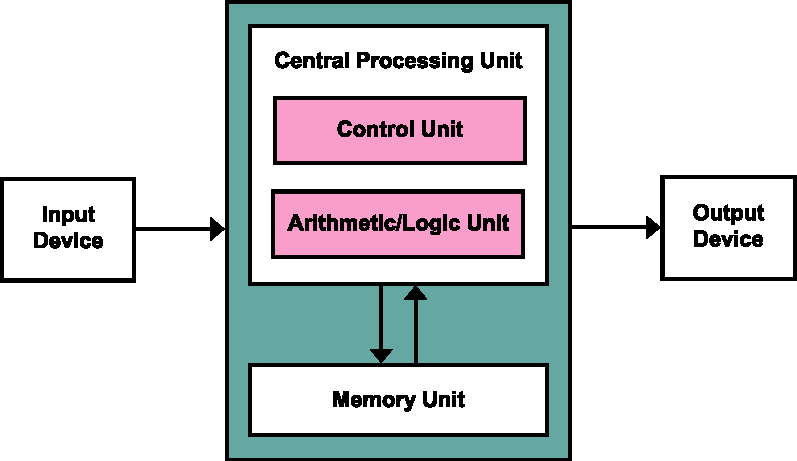
\includegraphics[width=10cm]{images/Von_Neumann_Architecture.pdf}
\\ \xxx{replace or properly attribute: Kapooht, 2013, CC BY-SA 3.0}
\end{center}

In a bottom up approach, this might also include the introduction of transistors, logic gates and circuits. In a top down approach, these could also be treated afterwards.

\subsection{Lesson Plan}
The goal of the lesson is for students to have connected their knowledge of high level programming with what happens within their machine when a program is executed.

If this is the student's encounter with Glamorous Toolkit, at least a brief introduction is in order (see \ref{ssc_lesson_gt}). Else we can directly start with a reminder of what they already know about programming.




\section{Further Lesson Ideas} \label{sc_lesson_other}
Connecting PA with Smalltalk; extend it to object oriented programming; mould the environment to questions developed during the course; ...

\chapter{Validation} \label{ch_practice}
% formerly: \texttt{PA} in Practice
PA has been used twice with students (on 2025-05-12 and 2025-06-30).

\section{First Round} \label{sc_validation_ca}
\subsection{Setting}

\begin{todo}
\item Own class, 14 students present, prepared according to prerequisites
\item Two lessons, afterwards questionnaire through Microsoft Forms
\end{todo}

\subsection{Observations}

\begin{todo}
\item adapt notes from gt-explorations
\end{todo}

\subsection{Student Feedback}
\subsection{Learnings}

\section{Second Round} \label{sc_validation_compiler}
\subsection{Setting}
\subsection{Observations}
\subsection{Student Feedback}
\subsection{Learnings}

%%%%% The Validation %%%%%

\chapter{Validation} \label{ch_practice}

The contents produced for this thesis have been used with two courses. Evaluation of the feedback provided by students show that they did like working with the provided environment and that their understanding of the abstractions involved in programming have increased somewhat. Due to limitations in the study setting, however further analysis will be required in order to generalize these findings.

Both courses were held with classes at Gymnasium Neufeld which we have been teaching ourselves for one and two years respectively. These classes consist of Swiss high school students at ninth and tenth grade (of twelve grades) respectively.


\section{First Round} \label{sc_validation_ca} % 2025-05-12

\subsection{Setting}

The first evaluation round took place in a computer science class consisting of 17 tenth grad students. This class had at this point encountered most of the base curriculum of computer science as required in the Canton of Berne \cite[p.\,145--146]{Erz16} with only the introduction to systems architecture missing.

Specifically, the introduction to programming had happened using Processing with Python syntax inside the Processing \ac{IDE}, so students had already the desired prior experience in programming with Processing. Additionally, the class had written their last partial exam five weeks prior which had among other topics contained a repetition sequence on binary numbers and encodings.

Contrary to the suggestions in \ref{sc_lesson_ca}, the introduction to computer architecture was happening bottom up, loosely following Nisan and Schocken's ideas \cite{Nis21} in a significantly abbreviated course of only 6 instead of 12 weeks.\footnote{The reason for this was originally the same as Nisan and Schocken's, \ie building concepts on a solid foundation.}

At the point where the environment developed for this thesis was introduced, students had already encountered some of the foundational building blocks of a modern microchip: transistors built out of semiconductors, logic gates and circuits up to an adder circuit as the basis of an \ac{ALU}.

The plan was thus to connect the already encountered foundation with their knowledge about programming by revealing and discussing several of the involved abstraction layers. Due to time constraints, only an excerpt of the sequence proposed in \ref{sc_lesson_ca} could be realized.

At the day of the lessons, 14 of the 17 students were present. At the start of the first lesson, \ac{GT} was distributed through the school's OneDrive infrastructure. The \ac{GT} environment was then introduced similar to \ref{ssc_lesson_gt} but, as was the rest of the lessons, mostly in a self-guided way with instructions being provided in \ac{GT} notebook pages.\footnote{The exact state of the materials is available at \url{https://github.com/zeniko/processing-abstractions/tree/thesis} in commit \ct{71047704f7f70c13d3d01ac520618e15d569274f} of May 12th.}

During the lessons, students were supported where needed but left to work at their own individual pace which the reduced number of students allowed for. Afterwards, a questionnaire\footnote{See appendix \ref{app_questionnaire_1} on page \pageref{app_questionnaire_1} for the full questionnaire.} was distributed to students for receiving their own feedback in addition to the collected observations.

At least one of the students missing the lessons was successfully able to work on the provided contents on her own.


\subsection{Observations}

During the time available, students have been able to work on their own for large amounts of time with only few common issues occurring. The interactive notebook pages seemed to allow for creating an effective teaching environment.

Additionally, many students have been observed to actively tinker with the interactive elements, as was desired and was to be expected from providing an environment for live programming and exploration. Except for a few hickups where the \ac{GT} notebook pages stopped updating (for which the usual cure of ``reloading'' helped), the interactivity worked reliably -- up to the point, where students found it so engaging that they got sidetracked by writing and modifying programs for their effect instead of the changes to the views for different layers.

Nonetheless, the more active students have been able to work through the subject matter on their own, whereas less interested students had to be motivated from time to time to continue reading and interacting. With students being able to work on their own, we had ample time for supporting these students with instructions, hints and some motivating background information.

Despite their prior Processing knowledge, students were sometimes out of their depth when changes to a Processing program were asked for. In a next round, this sequence would have to be placed closer to a programming sequence with Processing or at least a brief repetition of just using Processing would be helpful.

What caused most issues was the way \ac{GT} opened notebook pages from content links in a new page adjacent to the previous one, hiding the table of contents in the process, instead of opening them in place of the previous page as students were used to from webbrowsers. This caused students to lose track of on what pages they were supposed to be working, to the point of occasionally skipping part of the assigned content. This happened despite the brief introduction into working with \ac{GT} where closing additional pages and getting the table of contents back was an explicit introductionary task.

The overall impression of the lessons was that students had been working productively, mostly autonomously and at their own pace with the provided teaching materials.


\subsection{Student Feedback}

In order to verify our own observations, students were provided with a questionnaire for providing feedback. Of the 17 students, however only 11 returned feedback despite frequent reminding. The following yields thus at best qualitative results.\footnote{Questionnaire data in anonymized for is available at \url{https://github.com/zeniko/gyminf-thesis/blob/main/data/data_6_1.csv}.}

Additionally, three weeks later, the students have written another partial exam with individual tasks referring back to the lessons with \ac{GT}.

Student feedback shows the following: Students quite liked working with the provided environment (grading it in mostly 4/5) and reported that it worked reasonably well but not yet perfect (most students grading it either 3/5 or 4/5). This is consistent with our own observations.

Part of the reason for their liking working this way might be due to their noting programming (and one game programming project one year ago) as what they liked most about their computer science class with half the students naming this their ``highlight''.

When asked explicitly about the usefulness of the various abstraction views provided, students noted that they were very useful (mostly grading it either 4/5 or 5/5). Also, a majority of students indicated repeatedly actively interacting with the program samples.

What they liked the most was being able to work at their own speed (and optionally being able to decide for themselves whether to work together or alone) which is due to guidance from the environment which allows to introduce interactive tasks in place which students may explore autonomously in order to understand. One student explicitly noted that being able to see changes reflected instantly was gratifying.

Their main concern was two of the more engaged students noting that some explanations were not yet as clear as they could be, requiring them to ask instead of being able to work for themselves. Additionally, the quickest working student would have preferred fewer links within notebook pages, reducing the annoyance of losing the table of contents from webbrowser habits.

Students gave their feedback between one day and one week after the lesson. When asked to reword the learned content in their own words, most of them failed to describe what they'd learned entirely correctly. Would there answers have been graded, all but one students would have only been awarded at most half the points. Also, the desired connection with the previously taught contents about transistors and logic gates remained unclear with this time all students getting at most half the points.

Finally, the partial exam resulted in students answering questions related to these lessons only about 46\% correctly. The result does however weakly correlate with students' general commitment (measured by their final grade, yielding a rang correlation of $0.48$).


\subsection{Learnings}

The desired effects of having students better understand abstraction layers seems to not yet have been achieved. While the environment was engaging and led students to explore on their own, explanations will have to be expanded and made clearer for students to be able to fully understand what they're shown.

Part of the issue is however that time was too short and the implementation not fully fledged out, so these findings might also be due to both of these. So further analysis will be required and the environment will have to be tested at a larger scale with the other classes with better integration in the curriculum (as suggested by the author in \ref{sc_lesson_ca}).

At least some of the technical issues observed have since been remedied, although mostly by more explicitly telling students what to do when issues arise.

Also, since \ac{GT} runs purely on the student's own computers, their progress can't be observed other than by monitoring their screens. For this, either a separate progress tracker (such as \url{https://learningview.org/}) would have to be used or a sequence of short tests, not only checking for progress of reading but also of comprehension.



\section{Second Round} \label{sc_validation_compiler} % 2025-06-30

\subsection{Setting}

The second evaluation round took place in a computer science class consisting of 23 ninth grade students. This class had at that point passed about half the required contents of the base curriculum to computer science \cite[p.\,145--146]{Erz16}, including application usage, various encodings, algorithms and an introduction to programming using Processing eight weeks prior.\footnote{For timing reasons, unfortunately the programming project had to be postponed.}

Two lessons at the end of the school year could be set aside for an introduction to compilers as part of this thesis. These would usually have to be placed later in the curriculum, either together with the introduction to computer architecture or beyond.

The plan was to implement an excerpt of the course from \ref{sc_lesson_compiler}. As a quick overview, ``Human Resource Machine'' was used for introducing students to the limitations of machine language and motivating the need for compiling programs before executing them on actual hardware. Afterwards, \ac{GT} was introduced with additional stress on using the table of contents for navigation. Finally, students were asked to work through the provided contents at their own speed.\footnote{The exact state of the materials is available at \url{https://github.com/zeniko/processing-abstractions/tree/thesis} in commit \ct{6e22cddb176fdd46d410b9db40496bafa8a59c08} of June 30th.} Towards the end of the lessons, students were given time to fill out a questionnaire\footnote{See appendix \ref{app_questionnaire_2} on page \pageref{app_questionnaire_2} for the full questionnaire.}.

One unplanned limitation of these lessons were summer being early with high temperatures. As a consequence, only 15 of the 23 students were present for the introduction and the introduction had to be moved to a different, cooler location.


\subsection{Observations}

In general, the students worked reliably with the provided contents. In particular, this group seemed to quite naturally take notes within the \ac{GT} notebook pages, making the content their own.

Working speed again was heterogenous, but some smaller groups formed which supported each other. One student in particular volunteered repeatedly to help his peers.

Despite programming with Processing being rather fresh, fewer students seemed to interact with the sample programs provided, despite tasks asking them to do so explicitly. About half the students seemed content to observe views as static content.

This group had more problems getting \ac{GT} even to run. Even though these students had already successfully downloaded and used apps on their own, somehow despite a separate \ac{GT} launcher in the top level folder being provided, many failed to start \ac{GT} on their own.

Part of these issues might however relate to temperatures making it more difficult for students to focus.


\subsection{Student Feedback}

Of the 15 students present, 14 managed to hand in the questionnaire (with the last student's computer running out of battery).\footnote{Questionnaire data in anonymized for is available at \url{https://github.com/zeniko/gyminf-thesis/blob/main/data/data_6_2.csv}.} With this small number of answers, again no reasonable quantitative evaluation is possible.

The students answers show that many of them (12/15) have worked slower than expected, only learning about lexer and parser in the hour provided. Also, disappointingly only two of the 15 were at least somewhat confident that they would be able to explain the learned content to their peers.

This is consistent with students failing to answer basic questions about the need for compilation (half of them not answering or answering entirely wrong) but slightly better about the roles of lexer and parser (one third answering correctly and one third getting at least half of their answer correct).

It is difficult to judge how much of this is due to the environment not meeting expectations and how much is due to summer, as when asked directly about their thoughts of the provided environment, students wrongly referred ot the latter than the former.

The only general remark where students agreed on was that they had enjoyed programming (11/15) which however in contrast to the other class (see \ref{sc_validation_ca}) did not result in as much tinkering (with only 4/15 students reportedly playing around and exploring).


\subsection{Learnings}

Unfortunately, not much was to be learned from this test, mostly due to environmental factors. A repetition of this setting will thus be required at a later time. At least the content that students actually got to seems to have been sufficiently clear for them to somewhat understand.

%%%%% Conclusion and Future Work %%%%%

\chapter{Conclusion} \label{ch_conclusion}

In order to better understand complex content -- at least with regard to computer science --, didactic literature recommends that students perform a \emph{Sichtenwechsel}, \ie observe the same entity at different abstraction levels, in order to better understand the subject at hand. As part of our teaching computer science to high school students, we have been particularly interested in being able to do so with regards to programming, which is usually popular with students, and computer architecture, which tends to be less so.

While various programming \acp{IDE} provide some possibilities to get relevant insights into a computer's inner workings, none of them offer an all-in-one solution as a building block at a complexity level manageable for high school students. As part of this thesis, the new teaching environment Processing Abstractions has thus been introduced, implementing a compiler and runtime for the Processing language inside of \acf{GT}, which allows teachers to flexibly combine various forms of content in a unified environment. On the basis of the working Processing system, a wide variety of views of various aspects have been added, allowing students to inspect a program from source code to machine bytecode and along its execution.

This enabled the creation of interactive teaching material that engages students through its liveness and by allowing teachers to let them work at their own pace and depth through the material, having students explore and experience what steps computers have to take to transform their idea of a program into something sufficiently concrete that can be executed in a (virtual) machine.

Working with students showed that Processing Abstractions mostly worked and managed to get students involved. While students seem to have learned through their own investigation into lower abstraction levels, significant effects could not (yet) be measured. This was in large part due to both a small sample size and too brief an observation window.

Further usage and studies will be required to verify our initial assumptions. This is planned for the school years to come. Additionally, the foundational idea of abstraction levels has to be introduced alongside explicitly if students should be able to get a better understanding of when abstractions might leak and how that could be relevant.



\section{Future Work} \label{sc_future}

To continue further on this path, there are multiple ways to proceed. On the one hand, there are several aspects still missing from the environment itself. On the other hand, the same concept of \emph{Sichtenwechsel} might be applicable in other domains as well. Finally, a larger study confirming that this kind of approach is empirically sound is required.

Within the environment itself, there are several kinds of views that we feel are still missing. In particular, at this point, most views show a single state along abstraction deconstruction. Visualizations of the transitions from one to the next are still missing and would have to happen mainly in students' minds for now. Even just animating the Runsteps view instead of students having to click through, with differences from one step to the next being highlighted, might help. However, animating the process of parsing tokens into an \ac{AST} or, more ambitiously, the process of taking Processing source code, parsing it and then translating it would be more interesting.

Also, most lists provide access to native \ac{GT} objects, whose views are not optimized for students. Instead of \eg giving direct access to a bytecode object, which only contains a pointer back to the Smalltalk source, these could be wrapped or extended, so that their default view continues to be informative, such as showing a short explanation of what the selected command does.

In addition, the machine code shown to students is targeted at a stack machine. However, common microprocessors, such as those of the x64 architecture at the heart of our students' computers, are register-based. Compiling code to a matching machine language by \eg transpiling it to C and then having it compiled to x64 machine code would be a possible approach. Another approach would consist in directly translating it to Intel Assembly or corresponding bytecode. In order to then run such code, a matching virtual machine or a better way to show intermediary processor states would be required, if the execution steps are to be observed.

Two other steps that are missing for inspecting the process of compilation are type inference and optimizations. Processing and Smalltalk are both dynamically typed languages, which allows type checking considerations during the compilation to bytecode to be circumvented, as type differences are handled through inheritance and only optimized by a \ac{JIT}. Exposing type information and visualizing a type inference algorithm, such as Hindley-Milner, could be added. Python's syntax would even allow type hints, which could also be used to allow students to experiment with types.

Optimization, on the other hand, happens at various abstraction levels. With regard to choosing the right algorithm for a problem, a program's runtime behavior could be timed and shown. Alternatively, most programs written by high schoolers should be understandable and analyzable by current \acp{LLM}, so that adding a \ac{LLM}-enabled view could give students feedback at the highest level. At lower levels, \ac{GT} offers a \ct{GtMethodAdvice} system for analyzing source code at the method or expression level, which could be exposed and/or expanded. Similarly, \ac{GT}'s \ac{IR} could be optimized further than \ct{IrMethod>>optimize} does, and its optimization transformations could be exposed to students.

As for the implementation of Processing, many bits are missing. Mainly, support for object-oriented programming should be achievable, since Python's object model should again map sufficiently well onto Smalltalk's. What will, however, not be realistically possible is to get a sufficiently full Python inside \ac{GT}, which would allow importing (arbitrary) further modules. This should, however, not be as much of an issue, since similar to the Processing \ac{IDE}, hitting the limitations of the environment should be taken as a hint that the environment has been outgrown and to move to more capable tools, continuing the investigations using professional debuggers, memory viewers, \etc

For students coming from a different programming language, adapting the environment to their language of choice might also be doable. Since \ac{GT} already contains support for parsing dozens of languages (namely, among other languages, JavaScript, C(++), Rust, or even Visual Basic), matching a subset of that language from its \ac{AST} to Smalltalk should be doable in the same way as \ct{ProcessingTranspiler} was implemented. At least when sticking to the Processing \ac{API}, the rest of the environment could be reused with minimal adjustments.

Going beyond programming, the same principle might also be applicable to other domains: We have already seen the Filius environment, which allows students to deconstruct networks to various depths. In natural sciences, processes can be modeled, investigated and deconstructed in a similar fashion in a simulated environment. Based on a framework like NetLogo,\footnote{\emph{Cf.} \eg \url{https://www.netlogoweb.org/launch\#http://www.netlogoweb.org/assets/modelslib/Sample\%20Models/Biology/Ants.nlogo}.} which already presents multiple views of the same phenomenon, further views for deconstructing and understanding the observed behavior could be added. Having the simulation inside a moldable environment such as \ac{GT} would certainly help.

In the same vein, in a psychology course, students could be exposed to views of the subconscious, neurology down to biology and maybe even physics, when discussing behavior -- for a better understanding of the various influences on what might be perceived as purely mental; or in a music class, students could get harmonics decomposed into oscillation and ratios -- for a better understanding of what causes harmony; \etc Applying this principle in other domains is, however, left to the corresponding specialists. What is nonetheless desirable in all cases is an interdisciplinary approach once lower abstraction levels go beyond one's own domain.\footnote{Similarly to how chemistry and physics will have to be involved when discussing the innards of a modern microprocessor.}

However, first, we have to proceed with a further investigation into whether our students from different classes are indeed profiting in the way we intended them to -- by using Processing Abstractions for revealing programming language abstractions.


\appendix

%%%%% Technical Details %%%%%

\chapter{Installing and Using ``Processing Abstractions''} \label{app_setup}

In order to set up ``Processing Abstractions'', first download \ac{GT} from \url{https://gtoolkit.com/download/} for your platform and extract the archive's entire content.

Before running it, create a new text file called \ct{startup.st} in \ac{GT}'s top-level folder besides \ct{GlamorousToolkit.image} with the following content (access it through figure \ref{fig_startup_st_qr}):

\begin{code}
Metacello new
	repository: 'github://zeniko/\ac{GT}-exploration:thesis/src';
	baseline: 'GtExploration';
	load.

Metacello new
	repository: 'github://zeniko/processing-abstractions:thesis/src';
	baseline: 'ProcessingAbstractions';
	load.

"Hide the 'Implementation and Tests' section."
GtExplorationHomeSection studentMode: true.

"Make indenting keyboard shortcuts available to non-US-English keyboard layouts
(cf. https://github.com/feenkcom/gtoolkit/issues/3002)."
LeSnippetElement keyboardShortcuts
	at: #IndentSnippet
		put: BlKeyCombinationBuilder new alt shift arrowRight build;
	at: #UnindentSnippet
		put: BlKeyCombinationBuilder new alt shift arrowLeft build.

"Make the zoom in keyboard shortcut available to de-CH keyboard layouts
(cf. https://github.com/feenkcom/gtoolkit/issues/4624)."
TLeWithFontSize compile:
	((TLeWithFontSize methodNamed: #initializeFontSizeShortcuts) sourceCode
		copyReplaceAll: 'equal' with: 'shift minus').

"Patch unneeded addressbar out of YouTube snippet
(cf. https://github.com/feenkcom/gtoolkit/issues/4560)."
LeYoutubeReferenceElement compile:
	((LeYoutubeReferenceElement methodNamed: #updatePicture) sourceCode
		copyReplaceAll: '</iframe>'' ' with: '</iframe>''; removeChildAt: 1 ').
\end{code}

Finally run the \ct{GlamorousToolkit} executable (under Windows and Linux it's located in the \ct{bin} subfolder). The content of ``Processing Abstractions'' are now available behind the ``Unterrichtseinheiten'' home tile.

Verify that everything works as desired and then close and save the changes to the image. Now, the above \ct{startup.st} can be removed, since all its changes have been persisted in \ac{GT}'s \ct{.image} file.

\emph{Warning:} If you've already used \ac{GT} before, the contents of your local knowledge database will also be included in \ac{GT}'s image. Therefore rename that folder (usually \ct{lepiter/default} in your documents folder) before starting the \ac{GT} meant for distribution.

Also, since the executable \ct{GlamorousToolkit.exe} is located in a subdirectory under Windows and Linux, adding a top-level link can help students. See \url{https://github.com/zeniko/gtRunner} for a ready-to-use drop-in.

\begin{cfigure}[fig_startup_st_qr]{QR-link to the code for \ct{startup.st} for convenience}
\href{https://github.com/zeniko/gyminf-thesis/blob/main/appendix.tex}{
\includegraphics[height=2.5cm]{startup.st}}
\end{cfigure}



\chapter{GT Processing API} \label{app_api}

This appendix lists the available \ac{API} calls implemented in Processing Abstraction's Processing.\footnote{For comparison, the full \ac{API} or Processing's Python mode is available at \archivedurl{https://py.processing.org/reference/}.} This has been auto-generated from \ac{GT} page ``Processing API'':


\section{Rendering}

\subsection{Setup}
\begin{description}
\item[\texttt{background(r, g, b)}] \hfill \\
	Clears the canvas and changes its color (see \ct{fill(r, g, b)}). Default is light gray (192, 192, 192).
\item[\texttt{background(gray)}] \hfill \\
	Clears the canvas and changes its color (see \ct{fill(gray)}). Default is light gray (192).
\item[\texttt{size(width, height)}] \hfill \\
	Prepares an output canvas of the given dimensions. This command must always be called first (for animations: first command in \ct{def setup}).
\end{description}

\subsection{Shapes}
\begin{description}
\item[\texttt{circle(x, y, d)}] \hfill \\
	Draws a circle with the given diameter and its center at \ct{(x; y)}. Short for \ct{ellipse(x, y, d, d)}.
\item[\texttt{ellipse(x, y, dx, dy)}] \hfill \\
	Draws an ellipse with the given diameters and its center at \ct{(x; y)}.
\item[\texttt{image(image, x, y)}, \texttt{image(image, x, y, width, height)}] \hfill \\
	Renders the image loaded with \ct{loadImage(...)} at the given coordinates (and scales it to fit the given size). Arguments following after the first are identical to \ct{rect}'s. If \ct{width} and \ct{height} are not given, the image's native dimensions are used.
\item[\texttt{line(x1, y1, x2, y2)}] \hfill \\
	Draws a line from \ct{(x1; y1)} to \ct{(x2; y2)}.
\item[\texttt{loadImage(pathOrUrl)}] \hfill \\
	Loads the image from the given URL or path. The returned value is to be used with \ct{image(...)}.
Paths can be absolute or relative to either \ct{FileLocator class>>gtResource} or:
\begin{code}
Element
GtInspector newOn: FileLocator documents / 'lepiter'
\end{code}
\item[\texttt{rect(x, y, width, height)}, \texttt{rect(x, y, width, height, cornerRadius)}] \hfill \\
	Draws a rectangle of the given width and height, parallel to the coordinate axes with its top left corner at \ct{(x; y)}. Optionally round the corners, if a fifth argument is given.
\item[\texttt{square(x, y, side)}] \hfill \\
	Draws a square with the given side length, parallel to the coordinate axes with its top left corner at \ct{(x; y)}. Short for \ct{rect(x, y, side, side)}.
\item[\texttt{text(string, x, y)}] \hfill \\
	Renders the given \ct{string} with its baseline starting at \ct{(x; y)}.
\item[\texttt{textSize(size)}] \hfill \\
	Sets the size for rendering text in pixels. Default is 12px.
\item[\texttt{triangle(x1, y1, x2, y2, x3, y3)}] \hfill \\
	Draws a triangle with its vertices at the points \ct{(x1; y1)}, \ct{(x2; y2)} and \ct{(x3; y3)}.
\end{description}

\subsection{Colors}
\begin{description}
\item[\texttt{color(r, g, b)}, \texttt{color(gray)}] \hfill \\
	Generates a color object which can be stored in a variable also be used with \ct{fill(...)}, \ct{stroke(...)} and \ct{background(...)}.
\item[\texttt{fill(r, g, b)}] \hfill \\
	Selects the color to use for filling rendered shapes. The color is given as three values in the range of 0 to 255 (red, green and blue respectively). Default is white (255, 255, 255).
\item[\texttt{fill(gray)}] \hfill \\
	Selects the gray scale value to use for filling rendered shapes. The color is given as a single value in the range of 0 to 255 (black/dark to white/light). Default is white (255).
\item[\texttt{noStroke()}] \hfill \\
	Disables borders for future shapes. Equivalent to \ct{strokeWeight(0)}.
\item[\texttt{stroke(r, g, b)}] \hfill \\
	Selects the color to use for the borders of rendered shapes (see \ct{fill(r, g, b)}). Default is black (0, 0, 0).
\item[\texttt{stroke(gray)}] \hfill \\
	Selects the gray scale value to use for the borders of rendered shapes (see \ct{fill(gray)}). Default is black (0).
\item[\texttt{strokeWeight(weight)}] \hfill \\
	Determines the size of drawn borders in pixels. Default is 0.5px.
\end{description}

\subsection{Transforms}
\begin{description}
\item[\texttt{rotate(angle)}] \hfill \\
	Rotates all future shapes by the given angle (in \ct{radians}!) clockwise around the origin.
\item[\texttt{scale(factor)}] \hfill \\
	Linearly scales all future shapes by the given factor from the origin.
\item[\texttt{translate(x, y)}] \hfill \\
	Moves the origin \ct{(0; 0)} for all future shapes (defaults to the upper left corner).
\end{description}

\section{Events}
\begin{description}
\item[\texttt{def draw():}] \hfill \\
	is called repeatedly (up to \ct{frameRate} times per second) for drawing the output.
\item[\texttt{def mouseClicked():}] \hfill \\
	is called whenever a mouse button has been clicked \emph{and} released.
\item[\texttt{def mouseMoved():}] \hfill \\
	is called whenever the mouse has been moved. Alternatively query \ct{mouseX} and \ct{mouseY} in \ct{draw()}.
\item[\texttt{def mousePressed():}] \hfill \\
	is called whenever a mouse button has been pressed. Alternatively query \ct{mousePressed} in \ct{draw()}.
\item[\texttt{def mouseReleased():}] \hfill \\
	is called whenever a mouse button has been released.
\item[\texttt{def setup():}] \hfill \\
	is called once as the program starts.
\end{description}

\section{Mathematics}
\begin{description}
\item[\texttt{cos(angle)}] \hfill \\
	Returns the cosine value for the given angle (measured in radians).
\item[\texttt{int(value)}] \hfill \\
	Rounds the value to an integer.
\item[\texttt{PI}] \hfill \\
	The value of the mathematical constant p.
\item[\texttt{max(a, b)}] \hfill \\
	Returns the larger of the two values (\ct{max(a)} returns the largest value contained in the list \ct{a}).
\item[\texttt{min(a, b)}] \hfill \\
	Returns the smaller of the two values (\ct{min(a)} returns the smallest value contained in the list \ct{a}).
\item[\texttt{radians(angle)}] \hfill \\
	Converts the given angle (measured in degrees) into radians.
\item[\texttt{random(limit)}] \hfill \\
	Returns a random floating point number between 0 and limit (inclusive).
\item[\texttt{randomSeed(seed)}] \hfill \\
	Reinitializes the random generator with the given \ct{seed} number. Using the same number will result in the exact same sequence of pseudo-randomly generated numbers.
\item[\texttt{sin(angle)}] \hfill \\
	Returns the sine value for the given angle (measured in radians).
\item[\texttt{sq(value)}] \hfill \\
	Returns the squared value. Equivalent to \ct{value ** 2}
\item[\texttt{sqrt(value)}] \hfill \\
	Returns the square root of the given value.
\item[\texttt{tan(angle)}] \hfill \\
	Returns the tangent value for the given angle (measured in radians).
\end{description}

\section{Lists}
\begin{description}
\item[\texttt{append(list, value)}] \hfill \\
	Appends the value to the end of the list and returns \emph{a new} list (equivalent to \ct{list + [value]}).
(Note: \ct{list.append(...)} is \emph{not yet} supported.)
\item[\texttt{concat(list, otherList)}] \hfill \\
	Combines the two lists to a single \emph{new} list (equivalent to \ct{list + otherList}).
\item[\texttt{reversed(list)}] \hfill \\
	Returns a \emph{new} list with its content reversed.
(Note: \ct{list[::-1]} and \ct{list.reverse()} are \emph{not yet} supported.)
\item[\texttt{shorten(list)}] \hfill \\
	Returns a \emph{new} list without the last argument (equivalent to \ct{list[:-1]}).
\item[\texttt{sorted(list)}] \hfill \\
	Returns \emph{new} list with its content sorted.
(Note: \ct{list.sort()} is \emph{not yet} supported.)
\end{description}

\section{Miscellanea}
\begin{description}
\item[\texttt{delay(ms)}] \hfill \\
	Waits \ct{ms} milliseconds before continuing (mainly needed for demonstration purposes).
\item[\texttt{frameRate(fps)}] \hfill \\
	Limits the frame rate of animations to a maximum of \ct{fps} frames per second. Default is 30.
\item[\texttt{height}] \hfill \\
	Contains the canvas height as set by \ct{size()}.
\item[\texttt{millis()}] \hfill \\
	Returns the number of milliseconds that have passed since the program has started.
\item[\texttt{mouseX}, \texttt{mouseY}, \texttt{mousePressed}] \hfill \\
	Contains the \ct{x}- and \ct{y}-coordinates of the mouse cursor and whether the mouse has been pressed at the start of a \ct{draw}-phase (undefined outside of \ct{draw}).
\item[\texttt{print(value)}, \texttt{println(value)}] \hfill \\
	Prints the given value into an output console (mainly for debugging and for graphic-less program).
\item[\texttt{str(value)}] \hfill \\
	Turns the value into a string, e.\,g. for concatenating several values for use with \ct{text(...)}.
\item[\texttt{width}] \hfill \\
	Contains the canvas width as set by \ct{size()}.
\end{description}

\begin{todo}
\item Synchronize with \url{https://github.com/zeniko/\ac{GT}-exploration/blob/thesis/lepiter/68t44r92c7d0lr4e4ggiqmsq8.lepiter} and \url{https://github.com/zeniko/processing-abstractions/blob/thesis/lepiter/310yy5nuue5px1i3go4w0bjqo.lepiter}
\end{todo}




\chapter{Technical Implementation of ``Processing Abstractions''} \label{app_implementation}

\begin{cfigure}[fig_uml_snippet]{Diagram of classes involved in \ct{LeProcessingSnippet}}

\begin{tikzpicture}

\begin{package}{Snippet}

\begin{class}[text width=6.6cm]{LeProcessingSnippet}{0, 0}
\end{class}

\begin{class}[text width=6.6cm]{LeProcessingSnippetViewModel}{0, 2}
\end{class}

\begin{class}[text width=6.6cm]{LeProcessingSnippetElement}{0, 4}
\end{class}

\begin{class}[text width=6.6cm]{GtProcessingCoderModel}{8, 0}
\end{class}

\begin{class}[text width=6.6cm]{GtProcessingCoderViewModel}{8, 4}
\operation{doIt:}
\operation{doItAndGo:}
\operation{doItAndGoAsynchronous:}
\operation{doItAndGoSerialized:}
\operation{doItAndPublish:with:}
\end{class}

\draw[umlcd style dashed line, ->] (LeProcessingSnippet) -- node[black]{asSnippetViewModel} (LeProcessingSnippetViewModel);
\draw[umlcd style dashed line, ->] (LeProcessingSnippetViewModel) -- node[black]{snippetElementClass} (LeProcessingSnippetElement);
\draw[umlcd style dashed line, ->] (LeProcessingSnippet) -- node[black, rotate=90]{newCoder} (GtProcessingCoderModel);
\draw[umlcd style dashed line, ->] (GtProcessingCoderModel) -- node[black]{asCoderViewModel} (GtProcessingCoderViewModel);

\end{package}

\end{tikzpicture}

\end{cfigure}


%END Doc
%-------------------------------------------------------

\pagebreak % Abbreviations %%%%%%%%%%%%%%%%%%%%%%%%%%%%%%%%%%%%%%%%%%

\chapter*{Abbreviations}
\addcontentsline{toc}{chapter}{Abbreviations}

\begin{acronym}[REPL]
\acro{API}{Application Programming Interface}
\acro{ALU}{Arithmetic Logic Unit}
\acro{AST}{Abstract Syntax Tree}
\acro{CPU}{Central Processing Unit}
\acro{GT}{Glamorous Toolkit}
\acro{IDE}{Integrated Development Environment}
\acro{IR}{Intermediary Representation}
\acro{JIT}{Just-In Time Compiler}
\acro{JVM}{Java Virtual Machine}
\acro{LLM}{Large Language Model}
\acro{REPL}{Read-Evaluate-Print-Loop}
\acro{UI}{User Interface}
\acro{VM}{Virtual Machine}
\end{acronym}

\pagebreak % References %%%%%%%%%%%%%%%%%%%%%%%%%%%%%%%%%%%%%%%%%%

\addcontentsline{toc}{chapter}{Bibliography}

\bibliographystyle{plain}
\begin{raggedright}\bibliography{thesis}\end{raggedright}

\end{document}
